\documentclass[../main/NEMO_manual]{subfiles}

\begin{document}

\chapter{Ocean Tracers (TRA)}
\label{chap:TRA}

\thispagestyle{plain}

\chaptertoc

\paragraph{Changes record} ~\\

{\footnotesize
  \begin{tabularx}{\textwidth}{l||X|X}
    Release          & Author(s)                                   & Modifications       \\
    \hline
    {\em        4.0} & {\em Christian \'{E}th\'{e}               } & {\em Review       } \\
    {\em        3.6} & {\em Gurvan Madec                         } & {\em Update       } \\
    {\em $\leq$ 3.4} & {\em Gurvan Madec and S\'{e}bastien Masson} & {\em First version} \\
  \end{tabularx}
}

\clearpage

% missing/update
% traqsr: need to coordinate with SBC module

%STEVEN :  is the use of the word "positive" to describe a scheme enough, or should it be "positive definite"?
%I added a comment to this effect on some instances of this below

Using the representation described in \autoref{chap:DOM}, several semi -discrete space forms of
the tracer equations are available depending on the vertical coordinate used and on the physics used.
In all the equations presented here, the masking has been omitted for simplicity.
One must be aware that all the quantities are masked fields and that
each time a mean or difference operator is used, the resulting field is multiplied by a mask.

The two active tracers are potential temperature and salinity.
Their prognostic equations can be summarized as follows:
\[
  \text{NXT} =     \text{ADV} + \text{LDF} + \text{ZDF} + \text{SBC}
               + \{\text{QSR},  \text{BBC},  \text{BBL},  \text{DMP}\}
\]

NXT stands for next, referring to the time-stepping.
From left to right, the terms on the rhs of the tracer equations are the advection (ADV),
the lateral diffusion (LDF), the vertical diffusion (ZDF),
the contributions from the external forcings (SBC: Surface Boundary Condition,
QSR: penetrative Solar Radiation, and BBC: Bottom Boundary Condition),
the contribution from the bottom boundary Layer (BBL) parametrisation,
and an internal damping (DMP) term.
The terms QSR, BBC, BBL and DMP are optional.
The external forcings and parameterisations require complex inputs and complex calculations
(\eg\ bulk formulae, estimation of mixing coefficients) that are carried out in the SBC,
LDF and ZDF modules and described in \autoref{chap:SBC}, \autoref{chap:LDF} and
\autoref{chap:ZDF}, respectively.
Note that \mdl{tranpc}, the non-penetrative convection module,
although located in the \path{./src/OCE/TRA} directory as it directly modifies the tracer fields,
is described with the model vertical physics (ZDF) together with
other available parameterization of convection.

In the present chapter we also describe the diagnostic equations used to
compute the sea-water properties (density, Brunt-V\"{a}is\"{a}l\"{a} frequency, specific heat and
freezing point with associated modules \mdl{eosbn2} and \mdl{phycst}).

The different options available to the user are managed by namelist logicals.
For each equation term \textit{TTT}, the namelist logicals are \textit{ln\_traTTT\_xxx},
where \textit{xxx} is a 3 or 4 letter acronym corresponding to each optional scheme.
The equivalent code can be found in the \textit{traTTT} or \textit{traTTT\_xxx} module,
in the \path{./src/OCE/TRA} directory.

The user has the option of extracting each tendency term on the RHS of the tracer equation for output
(\np{ln_tra_trd}{ln\_tra\_trd} or \np[=.true.]{ln_tra_mxl}{ln\_tra\_mxl}),
as described in \autoref{chap:DIA}.

%% =================================================================================================
\section[Tracer advection (\textit{traadv.F90})]{Tracer advection (\protect\mdl{traadv})}
\label{sec:TRA_adv}

\begin{listing}
  \nlst{namtra_adv}
  \caption{\forcode{&namtra_adv}}
  \label{lst:namtra_adv}
\end{listing}

When considered (\ie\ when \np{ln_traadv_OFF}{ln\_traadv\_OFF} is not set to \forcode{.true.}),
the advection tendency of a tracer is expressed in flux form,
\ie\ as the divergence of the advective fluxes.
Its discrete expression is given by:
\begin{equation}
  \label{eq:TRA_adv}
  ADV_\tau = - \frac{1}{b_t} \Big(   \delta_i [ e_{2u} \, e_{3u} \; u \; \tau_u]
                                   + \delta_j [ e_{1v} \, e_{3v} \; v \; \tau_v] \Big)
             - \frac{1}{e_{3t}} \delta_k [w \; \tau_w]
\end{equation}
where $\tau$ is either T or S, and $b_t = e_{1t} \, e_{2t} \, e_{3t}$ is the volume of $T$-cells.
The flux form in \autoref{eq:TRA_adv} implicitly requires the use of the continuity equation.
Indeed, it is obtained by using the following equality:
$\nabla \cdot (\vect U \, T) = \vect U \cdot \nabla T$ which
results from the use of the continuity equation,
$\partial_t e_3 + e_3 \; \nabla \cdot \vect U = 0$
(which reduces to $\nabla \cdot \vect U = 0$ in linear free surface,
\ie\ \np[=.true.]{ln_linssh}{ln\_linssh}).
Therefore it is of paramount importance to
design the discrete analogue of the advection tendency so that
it is consistent with the continuity equation in order to
enforce the conservation properties of the continuous equations.
In other words, by setting $\tau = 1$ in (\autoref{eq:TRA_adv}) we recover
the discrete form of the continuity equation which is used to calculate the vertical velocity.
\begin{figure}
  \centering
  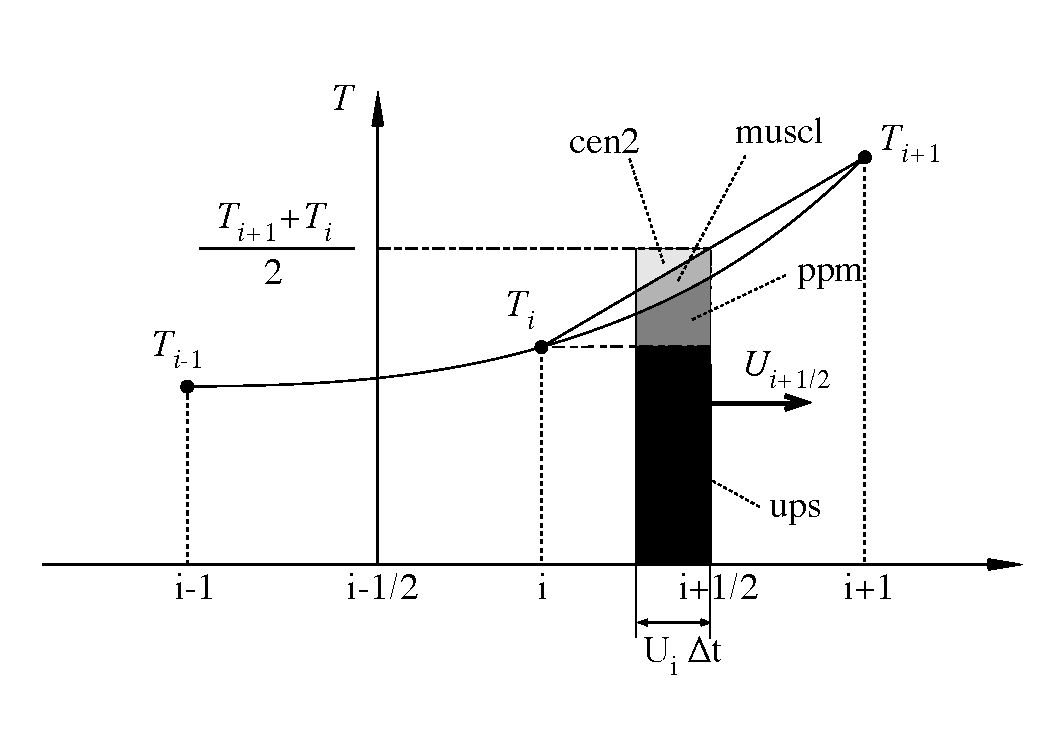
\includegraphics[width=0.66\textwidth]{TRA_adv_scheme}
  \caption[Ways to evaluate the tracer value and the amount of tracer exchanged]{
    Schematic representation of some ways used to evaluate the tracer value at $u$-point and
    the amount of tracer exchanged between two neighbouring grid points.
    Upsteam biased scheme (ups):
    the upstream value is used and the black area is exchanged.
    Piecewise parabolic method (ppm):
    a parabolic interpolation is used and the black and dark grey areas are exchanged.
    Monotonic upstream scheme for conservative laws (muscl):
    a parabolic interpolation is used and black, dark grey and grey areas are exchanged.
    Second order scheme (cen2):
    the mean value is used and black, dark grey, grey and light grey areas are exchanged.
    Note that this illustration does not include the flux limiter used in ppm and muscl schemes.}
  \label{fig:TRA_adv_scheme}
\end{figure}

The key difference between the advection schemes available in \NEMO\ is the choice made in
space and time interpolation to define the value of the tracer at the velocity points
(\autoref{fig:TRA_adv_scheme}).

Along solid lateral and bottom boundaries a zero tracer flux is automatically specified,
since the normal velocity is zero there.
At the sea surface the boundary condition depends on the type of sea surface chosen:

\begin{description}
\item [linear free surface] (\np[=.true.]{ln_linssh}{ln\_linssh})
  the first level thickness is constant in time:
  the vertical boundary condition is applied at the fixed surface $z = 0$ rather than
  on the moving surface $z = \eta$.
  There is a non-zero advective flux which is set for
  all advection schemes as $\tau_w|_{k = 1/2} = T_{k = 1}$,
  \ie\ the product of surface velocity (at $z = 0$) by the first level tracer value.
\item [non-linear free surface] (\np[=.false.]{ln_linssh}{ln\_linssh})
  convergence/divergence in the first ocean level moves the free surface up/down.
  There is no tracer advection through it so that
  the advective fluxes through the surface are also zero.
\end{description}

In all cases, this boundary condition retains local conservation of tracer.
Global conservation is obtained in non-linear free surface case,
but \textit{not} in the linear free surface case.
Nevertheless, in the latter case,
it is achieved to a good approximation since the non-conservative term is
the product of the time derivative of the tracer and the free surface height,
two quantities that are not correlated
\citep{roullet.madec_JGR00, griffies.pacanowski.ea_MWR01, campin.adcroft.ea_OM04}.

The velocity field that appears in (\autoref{eq:TRA_adv} is
the centred (\textit{now}) \textit{effective} ocean velocity, \ie\ the \textit{eulerian} velocity
(see \autoref{chap:DYN}) plus the eddy induced velocity (\textit{eiv}) and/or
the mixed layer eddy induced velocity (\textit{eiv}) when those parameterisations are used
(see \autoref{chap:LDF}).

Several tracer advection scheme are proposed,
namely a $2^{nd}$ or $4^{th}$ order \textbf{CEN}tred schemes (CEN),
a $2^{nd}$ or $4^{th}$ order \textbf{F}lux \textbf{C}orrected \textbf{T}ransport scheme (FCT),
a \textbf{M}onotone \textbf{U}pstream \textbf{S}cheme for
\textbf{C}onservative \textbf{L}aws scheme (MUSCL),
a $3^{rd}$ \textbf{U}pstream \textbf{B}iased \textbf{S}cheme (UBS, also often called UP3),
and a \textbf{Q}uadratic \textbf{U}pstream \textbf{I}nterpolation for
\textbf{C}onvective \textbf{K}inematics with
\textbf{E}stimated \textbf{S}treaming \textbf{T}erms scheme (QUICKEST).
The choice is made in the \nam{tra_adv}{tra\_adv} namelist,
by setting to \forcode{.true.} one of the logicals \textit{ln\_traadv\_xxx}.
The corresponding code can be found in the \textit{traadv\_xxx.F90} module,
where \textit{xxx} is a 3 or 4 letter acronym corresponding to each scheme.
By default (\ie\ in the reference namelist, \textit{namelist\_ref}),
all the logicals are set to \forcode{.false.}.
If the user does not select an advection scheme in the configuration namelist
(\textit{namelist\_cfg}), the tracers will \textit{not} be advected!

Details of the advection schemes are given below.
The choosing an advection scheme is a complex matter which depends on the
model physics, model resolution, type of tracer, as well as the issue of numerical cost.
In particular, we note that

\begin{enumerate}
\item CEN and FCT schemes require an explicit diffusion operator while
  the other schemes are diffusive enough so that they do not necessarily need additional diffusion;
\item CEN and UBS are not \textit{positive} schemes \footnote{negative values can appear in
    an initially strictly positive tracer field which is advected},
  implying that false extrema are permitted.
  Their use is not recommended on passive tracers;
\item It is recommended that the same advection-diffusion scheme is used on
  both active and passive tracers.
\end{enumerate}

Indeed, if a source or sink of a passive tracer depends on an active one,
the difference of treatment of active and passive tracers can create
very nice-looking frontal structures that are pure numerical artefacts.
Nevertheless, most of our users set a different treatment on passive and active tracers,
that's the reason why this possibility is offered.
We strongly suggest them to perform a sensitivity experiment using a same treatment to
assess the robustness of their results.

%% =================================================================================================
\subsection[CEN: Centred scheme (\forcode{ln_traadv_cen})]{CEN: Centred scheme (\protect\np{ln_traadv_cen}{ln\_traadv\_cen})}
\label{subsec:TRA_adv_cen}

%        2nd order centred scheme

The \textbf{CEN}tred advection scheme (CEN) is used when \np[=.true.]{ln_traadv_cen}{ln\_traadv\_cen}.
Its order ($2^{nd}$ or $4^{th}$) can be chosen independently on
horizontal (iso-level) and vertical direction by
setting \np{nn_cen_h}{nn\_cen\_h} and \np{nn_cen_v}{nn\_cen\_v} to $2$ or $4$.
CEN implementation can be found in the \mdl{traadv\_cen} module.

In the $2^{nd}$ order centred formulation (CEN2), the tracer at velocity points is evaluated as
the mean of the two neighbouring $T$-point values.
For example, in the $i$-direction :
\begin{equation}
  \label{eq:TRA_adv_cen2}
  \tau_u^{cen2} = \overline T ^{i + 1/2}
\end{equation}

CEN2 is non diffusive (\ie\ it conserves the tracer variance, $\tau^2$) but
dispersive (\ie\ it may create false extrema).
It is therefore notoriously noisy and must be used in conjunction with
an explicit diffusion operator to produce a sensible solution.
The associated time-stepping is performed using
a leapfrog scheme in conjunction with an Asselin time-filter,
so $T$ in (\autoref{eq:TRA_adv_cen2}) is the \textit{now} tracer value.

Note that using the CEN2, the overall tracer advection is of second order accuracy since
both (\autoref{eq:TRA_adv}) and (\autoref{eq:TRA_adv_cen2}) have this order of accuracy.

%        4nd order centred scheme

In the $4^{th}$ order formulation (CEN4),
tracer values are evaluated at u- and v-points as a $4^{th}$ order interpolation,
and thus depend on the four neighbouring $T$-points.
For example, in the $i$-direction:
\begin{equation}
  \label{eq:TRA_adv_cen4}
  \tau_u^{cen4} = \overline{T - \frac{1}{6} \, \delta_i \Big[ \delta_{i + 1/2}[T] \, \Big]}^{\,i + 1/2}
\end{equation}
In the vertical direction (\np[=4]{nn_cen_v}{nn\_cen\_v}),
a $4^{th}$ COMPACT interpolation has been prefered \citep{demange_phd14}.
In the COMPACT scheme, both the field and its derivative are interpolated,
which leads, after a matrix inversion, spectral characteristics similar to schemes of higher order
\citep{lele_JCP92}.

Strictly speaking, the CEN4 scheme is not a $4^{th}$ order advection scheme but
a $4^{th}$ order evaluation of advective fluxes,
since the divergence of advective fluxes \autoref{eq:TRA_adv} is kept at $2^{nd}$ order.
The expression \textit{$4^{th}$ order scheme} used in oceanographic literature is
usually associated with the scheme presented here.
Introducing a ``true'' $4^{th}$ order advection scheme is feasible but, for consistency reasons,
it requires changes in the discretisation of the tracer advection together with
changes in the continuity equation, and the momentum advection and pressure terms.

A direct consequence of the pseudo-fourth order nature of the scheme is that it is not non-diffusive,
\ie\ the global variance of a tracer is not preserved using CEN4.
Furthermore, it must be used in conjunction with an explicit diffusion operator to
produce a sensible solution.
As in CEN2 case, the time-stepping is performed using a leapfrog scheme in conjunction with
an Asselin time-filter, so $T$ in (\autoref{eq:TRA_adv_cen4}) is the \textit{now} tracer.

At a $T$-grid cell adjacent to a boundary (coastline, bottom and surface),
an additional hypothesis must be made to evaluate $\tau_u^{cen4}$.
This hypothesis usually reduces the order of the scheme.
Here we choose to set the gradient of $T$ across the boundary to zero.
Alternative conditions can be specified,
such as a reduction to a second order scheme for these near boundary grid points.

%% =================================================================================================
\subsection[FCT: Flux Corrected Transport scheme (\forcode{ln_traadv_fct})]{FCT: Flux Corrected Transport scheme (\protect\np{ln_traadv_fct}{ln\_traadv\_fct})}
\label{subsec:TRA_adv_tvd}

The \textbf{F}lux \textbf{C}orrected \textbf{T}ransport schemes (FCT) is used when
\np[=.true.]{ln_traadv_fct}{ln\_traadv\_fct}.
Its order ($2^{nd}$ or $4^{th}$) can be chosen independently on
horizontal (iso-level) and vertical direction by
setting \np{nn_fct_h}{nn\_fct\_h} and \np{nn_fct_v}{nn\_fct\_v} to $2$ or $4$.
FCT implementation can be found in the \mdl{traadv\_fct} module.

In FCT formulation, the tracer at velocity points is evaluated using
a combination of an upstream and a centred scheme.
For example, in the $i$-direction :
\begin{equation}
  \label{eq:TRA_adv_fct}
  \begin{split}
    \tau_u^{ups} &=
    \begin{cases}
                     T_{i + 1} & \text{if~} u_{i + 1/2} <    0 \\
                     T_i       & \text{if~} u_{i + 1/2} \geq 0 \\
    \end{cases} \\
    \tau_u^{fct} &= \tau_u^{ups} + c_u \, \big( \tau_u^{cen} - \tau_u^{ups} \big)
  \end{split}
\end{equation}
where $c_u$ is a flux limiter function taking values between 0 and 1.
The FCT order is the one of the centred scheme used
(\ie\ it depends on the setting of \np{nn_fct_h}{nn\_fct\_h} and \np{nn_fct_v}{nn\_fct\_v}).
There exist many ways to define $c_u$, each corresponding to a different FCT scheme.
The one chosen in \NEMO\ is described in \citet{zalesak_JCP79}.
$c_u$ only departs from $1$ when the advective term produces a local extremum in the tracer field.
The resulting scheme is quite expensive but \textit{positive}.
It can be used on both active and passive tracers.
A comparison of FCT-2 with MUSCL and a MPDATA scheme can be found in \citet{levy.estublier.ea_GRL01}.

For stability reasons (see \autoref{chap:TD}),
$\tau_u^{cen}$ is evaluated in (\autoref{eq:TRA_adv_fct}) using the \textit{now} tracer while
$\tau_u^{ups}$ is evaluated using the \textit{before} tracer.
In other words, the advective part of the scheme is time stepped with a leap-frog scheme while
a forward scheme is used for the diffusive part.

%% =================================================================================================
\subsection[MUSCL: Monotone Upstream Scheme for Conservative Laws (\forcode{ln_traadv_mus})]{MUSCL: Monotone Upstream Scheme for Conservative Laws (\protect\np{ln_traadv_mus}{ln\_traadv\_mus})}
\label{subsec:TRA_adv_mus}

The \textbf{M}onotone \textbf{U}pstream \textbf{S}cheme for \textbf{C}onservative \textbf{L}aws
(MUSCL) is used when \np[=.true.]{ln_traadv_mus}{ln\_traadv\_mus}.
MUSCL implementation can be found in the \mdl{traadv\_mus} module.

MUSCL has been first implemented in \NEMO\ by \citet{levy.estublier.ea_GRL01}.
In its formulation, the tracer at velocity points is evaluated assuming
a linear tracer variation between two $T$-points (\autoref{fig:TRA_adv_scheme}).
For example, in the $i$-direction :
\[
  % \label{eq:TRA_adv_mus}
  \tau_u^{mus} = \lt\{
  \begin{split}
    \tau_i        &+ \frac{1}{2} \lt( 1 - \frac{u_{i + 1/2} \, \rdt}{e_{1u}} \rt)
    \widetilde{\partial_i        \tau} & \text{if~} u_{i + 1/2} \geqslant 0 \\
    \tau_{i + 1/2} &+ \frac{1}{2} \lt( 1 + \frac{u_{i + 1/2} \, \rdt}{e_{1u}} \rt)
    \widetilde{\partial_{i + 1/2} \tau} & \text{if~} u_{i + 1/2} <         0
  \end{split}
                                                                                                      \rt.
\]
where $\widetilde{\partial_i \tau}$ is the slope of the tracer on which
a limitation is imposed to ensure the \textit{positive} character of the scheme.

The time stepping is performed using a forward scheme,
that is the \textit{before} tracer field is used to evaluate $\tau_u^{mus}$.

For an ocean grid point adjacent to land and where the ocean velocity is directed toward land,
an upstream flux is used.
This choice ensure the \textit{positive} character of the scheme.
In addition, fluxes round a grid-point where a runoff is applied can optionally be computed using
upstream fluxes (\np[=.true.]{ln_mus_ups}{ln\_mus\_ups}).

%% =================================================================================================
\subsection[UBS a.k.a. UP3: Upstream-Biased Scheme (\forcode{ln_traadv_ubs})]{UBS a.k.a. UP3: Upstream-Biased Scheme (\protect\np{ln_traadv_ubs}{ln\_traadv\_ubs})}
\label{subsec:TRA_adv_ubs}

The \textbf{U}pstream-\textbf{B}iased \textbf{S}cheme (UBS) is used when
\np[=.true.]{ln_traadv_ubs}{ln\_traadv\_ubs}.
UBS implementation can be found in the \mdl{traadv\_mus} module.

The UBS scheme, often called UP3, is also known as the Cell Averaged QUICK scheme
(\textbf{Q}uadratic \textbf{U}pstream \textbf{I}nterpolation for
\textbf{C}onvective \textbf{K}inematics).
It is an upstream-biased third order scheme based on an upstream-biased parabolic interpolation.
For example, in the $i$-direction:
\begin{equation}
  \label{eq:TRA_adv_ubs}
  \tau_u^{ubs} = \overline T ^{i + 1/2} - \frac{1}{6}
    \begin{cases}
      \tau"_i       & \text{if~} u_{i + 1/2} \geqslant 0 \\
      \tau"_{i + 1} & \text{if~} u_{i + 1/2} <         0
    \end{cases}
  \quad \text{where~} \tau"_i = \delta_i \lt[ \delta_{i + 1/2} [\tau] \rt]
\end{equation}

This results in a dissipatively dominant (i.e. hyper-diffusive) truncation error
\citep{shchepetkin.mcwilliams_OM05}.
The overall performance of the advection scheme is similar to that reported in
\cite{farrow.stevens_JPO95}.
It is a relatively good compromise between accuracy and smoothness.
Nevertheless the scheme is not \textit{positive}, meaning that false extrema are permitted,
but the amplitude of such are significantly reduced over the centred second or fourth order method.
Therefore it is not recommended that it should be applied to
a passive tracer that requires positivity.

The intrinsic diffusion of UBS makes its use risky in the vertical direction where
the control of artificial diapycnal fluxes is of paramount importance
\citep{shchepetkin.mcwilliams_OM05, demange_phd14}.
Therefore the vertical flux is evaluated using either a $2^nd$ order FCT scheme or
a $4^th$ order COMPACT scheme (\np[=2 or 4]{nn_ubs_v}{nn\_ubs\_v}).

For stability reasons (see \autoref{chap:TD}),
the first term  in \autoref{eq:TRA_adv_ubs} (which corresponds to a second order centred scheme)
is evaluated using the \textit{now}    tracer (centred in time) while
the second term (which is the diffusive part of the scheme),
is evaluated using the \textit{before} tracer (forward in time).
This choice is discussed by \citet{webb.de-cuevas.ea_JAOT98} in
the context of the QUICK advection scheme.
UBS and QUICK schemes only differ by one coefficient.
Replacing 1/6 with 1/8 in \autoref{eq:TRA_adv_ubs} leads to the QUICK advection scheme
\citep{webb.de-cuevas.ea_JAOT98}.
This option is not available through a namelist parameter, since the 1/6 coefficient is hard coded.
Nevertheless it is quite easy to make the substitution in the \mdl{traadv\_ubs} module and
obtain a QUICK scheme.

Note that it is straightforward to rewrite \autoref{eq:TRA_adv_ubs} as follows:
\begin{gather}
  \label{eq:TRA_adv_ubs2}
  \tau_u^{ubs} = \tau_u^{cen4} + \frac{1}{12}
    \begin{cases}
      + \tau"_i       & \text{if} \ u_{i + 1/2} \geqslant 0 \\
      - \tau"_{i + 1} & \text{if} \ u_{i + 1/2} <         0
    \end{cases}
  \intertext{or equivalently}
  % \label{eq:TRA_adv_ubs2b}
  u_{i + 1/2} \ \tau_u^{ubs} = u_{i + 1/2} \, \overline{T - \frac{1}{6} \, \delta_i \Big[ \delta_{i + 1/2}[T] \Big]}^{\,i + 1/2}
                             - \frac{1}{2} |u|_{i + 1/2} \, \frac{1}{6} \, \delta_{i + 1/2} [\tau"_i] \nonumber
\end{gather}

\autoref{eq:TRA_adv_ubs2} has several advantages.
Firstly, it clearly reveals that the UBS scheme is based on the fourth order scheme to which
an upstream-biased diffusion term is added.
Secondly,
this emphasises that the $4^{th}$ order part (as well as the $2^{nd}$ order part as stated above) has to be evaluated at the \textit{now} time step using \autoref{eq:TRA_adv_ubs}.
Thirdly, the diffusion term is in fact a biharmonic operator with
an eddy coefficient which is simply proportional to the velocity:
$A_u^{lm} = \frac{1}{12} \, {e_{1u}}^3 \, |u|$.
Note the current version of \NEMO\ uses the computationally more efficient formulation
\autoref{eq:TRA_adv_ubs}.

%% =================================================================================================
\subsection[QCK: QuiCKest scheme (\forcode{ln_traadv_qck})]{QCK: QuiCKest scheme (\protect\np{ln_traadv_qck}{ln\_traadv\_qck})}
\label{subsec:TRA_adv_qck}

The \textbf{Q}uadratic \textbf{U}pstream \textbf{I}nterpolation for
\textbf{C}onvective \textbf{K}inematics with \textbf{E}stimated \textbf{S}treaming \textbf{T}erms
(QUICKEST) scheme proposed by \citet{leonard_CMAME79} is used when
\np[=.true.]{ln_traadv_qck}{ln\_traadv\_qck}.
QUICKEST implementation can be found in the \mdl{traadv\_qck} module.

QUICKEST is the third order Godunov scheme which is associated with the ULTIMATE QUICKEST limiter
\citep{leonard_CMAME91}.
It has been implemented in \NEMO\ by G. Reffray (Mercator Ocean) and
can be found in the \mdl{traadv\_qck} module.
The resulting scheme is quite expensive but \textit{positive}.
It can be used on both active and passive tracers.
However, the intrinsic diffusion of QCK makes its use risky in the vertical direction where
the control of artificial diapycnal fluxes is of paramount importance.
Therefore the vertical flux is evaluated using the CEN2 scheme.
This no longer guarantees the positivity of the scheme.
The use of FCT in the vertical direction (as for the UBS case) should be implemented to
restore this property.

\cmtgm{Cross term are missing in the current implementation....}

%% =================================================================================================
\section[Tracer lateral diffusion (\textit{traldf.F90})]{Tracer lateral diffusion (\protect\mdl{traldf})}
\label{sec:TRA_ldf}

\begin{listing}
  \nlst{namtra_ldf}
  \caption{\forcode{&namtra_ldf}}
  \label{lst:namtra_ldf}
\end{listing}

Options are defined through the \nam{tra_ldf}{tra\_ldf} namelist variables.
They are regrouped in four items, allowing to specify
\begin{enumerate*}[label=(\textit{\roman*})]
\item the type of operator used (none, laplacian, bilaplacian),
\item the direction along which the operator acts (iso-level, horizontal, iso-neutral),
\item some specific options related to the rotated operators (\ie\ non-iso-level operator), and
\item the specification of eddy diffusivity coefficient
  (either constant or variable in space and time).
\end{enumerate*}
Item (iv) will be described in \autoref{chap:LDF}.
The direction along which the operators act is defined through the slope between
this direction and the iso-level surfaces.
The slope is computed in the \mdl{ldfslp} module and will also be described in \autoref{chap:LDF}.

The lateral diffusion of tracers is evaluated using a forward scheme,
\ie\ the tracers appearing in its expression are the \textit{before} tracers in time,
except for the pure vertical component that appears when a rotation tensor is used.
This latter component is solved implicitly together with the vertical diffusion term
(see \autoref{chap:TD}).
When \np[=.true.]{ln_traldf_msc}{ln\_traldf\_msc},
a Method of Stabilizing Correction is used in which the pure vertical component is split into
an explicit and an implicit part \citep{lemarie.debreu.ea_OM12}.

%% =================================================================================================
\subsection[Type of operator (\forcode{ln_traldf_}\{\forcode{OFF,lap,blp}\})]{Type of operator (\protect\np{ln_traldf_OFF}{ln\_traldf\_OFF}, \protect\np{ln_traldf_lap}{ln\_traldf\_lap}, or \protect\np{ln_traldf_blp}{ln\_traldf\_blp})}
\label{subsec:TRA_ldf_op}

Three operator options are proposed and, one and only one of them must be selected:

\begin{description}
\item [{\np[=.true.]{ln_traldf_OFF}{ln\_traldf\_OFF}}] no operator selected,
  the lateral diffusive tendency will not be applied to the tracer equation.
  This option can be used when the selected advection scheme is diffusive enough
  (MUSCL scheme for example).
\item [{\np[=.true.]{ln_traldf_lap}{ln\_traldf\_lap}}] a laplacian operator is selected.
  This harmonic operator takes the following expression:
  $\mathcal{L}(T) = \nabla \cdot A_{ht} \; \nabla T $,
  where the gradient operates along the selected direction (see \autoref{subsec:TRA_ldf_dir}),
  and $A_{ht}$ is the eddy diffusivity coefficient expressed in $m^2/s$ (see \autoref{chap:LDF}).
\item [{\np[=.true.]{ln_traldf_blp}{ln\_traldf\_blp}}] a bilaplacian operator is selected.
  This biharmonic operator takes the following expression:
  $\mathcal{B} = - \mathcal{L}(\mathcal{L}(T)) = - \nabla \cdot b \nabla (\nabla \cdot b \nabla T)$
  where the gradient operats along the selected direction,
  and $b^2 = B_{ht}$ is the eddy diffusivity coefficient expressed in $m^4/s$
  (see \autoref{chap:LDF}).
  In the code, the bilaplacian operator is obtained by calling the laplacian twice.
\end{description}

Both laplacian and bilaplacian operators ensure the total tracer variance decrease.
Their primary role is to provide strong dissipation at the smallest scale supported by the grid while
minimizing the impact on the larger scale features.
The main difference between the two operators is the scale selectiveness.
The bilaplacian damping time (\ie\ its spin down time) scales like
$\lambda^{-4}$ for disturbances of wavelength $\lambda$
(so that short waves damped more rapidelly than long ones),
whereas the laplacian damping time scales only like $\lambda^{-2}$.

%% =================================================================================================
\subsection[Action direction (\forcode{ln_traldf_}\{\forcode{lev,hor,iso,triad}\})]{Direction of action (\protect\np{ln_traldf_lev}{ln\_traldf\_lev}, \protect\np{ln_traldf_hor}{ln\_traldf\_hor}, \protect\np{ln_traldf_iso}{ln\_traldf\_iso}, or \protect\np{ln_traldf_triad}{ln\_traldf\_triad})}
\label{subsec:TRA_ldf_dir}

The choice of a direction of action determines the form of operator used.
The operator is a simple (re-entrant) laplacian acting in the (\textbf{i},\textbf{j}) plane when
iso-level option is used (\np[=.true.]{ln_traldf_lev}{ln\_traldf\_lev}) or when
a horizontal (\ie\ geopotential) operator is demanded in \textit{z}-coordinate
(\np{ln_traldf_hor}{ln\_traldf\_hor} and \np[=.true.]{ln_zco}{ln\_zco}).
The associated code can be found in the \mdl{traldf\_lap\_blp} module.
The operator is a rotated (re-entrant) laplacian when
the direction along which it acts does not coincide with the iso-level surfaces,
that is when standard or triad iso-neutral option is used
(\np{ln_traldf_iso}{ln\_traldf\_iso} or \np{ln_traldf_triad}{ln\_traldf\_triad} = \forcode{.true.},
see \mdl{traldf\_iso} or \mdl{traldf\_triad} module, resp.), or
when a horizontal (\ie\ geopotential) operator is demanded in \textit{s}-coordinate
(\np{ln_traldf_hor}{ln\_traldf\_hor} and \np{ln_sco}{ln\_sco} = \forcode{.true.}) \footnote{
  In this case, the standard iso-neutral operator will be automatically selected}.
In that case, a rotation is applied to the gradient(s) that appears in the operator so that
diffusive fluxes acts on the three spatial direction.

The resulting discret form of the three operators (one iso-level and two rotated one) is given in
the next two sub-sections.

%% =================================================================================================
\subsection[Iso-level (bi-)laplacian operator (\forcode{ln_traldf_iso})]{Iso-level (bi-)laplacian operator ( \protect\np{ln_traldf_iso}{ln\_traldf\_iso})}
\label{subsec:TRA_ldf_lev}

The laplacian diffusion operator acting along the model (\textit{i,j})-surfaces is given by:
\begin{equation}
  \label{eq:TRA_ldf_lap}
  D_t^{lT} = \frac{1}{b_t} \Bigg(   \delta_{i} \lt[ A_u^{lT} \; \frac{e_{2u} \, e_{3u}}{e_{1u}} \; \delta_{i + 1/2} [T] \rt]
                                  + \delta_{j} \lt[ A_v^{lT} \; \frac{e_{1v} \, e_{3v}}{e_{2v}} \; \delta_{j + 1/2} [T] \rt] \Bigg)
\end{equation}
where $b_t = e_{1t} \, e_{2t} \, e_{3t}$  is the volume of $T$-cells and
where zero diffusive fluxes is assumed across solid boundaries,
first (and third in bilaplacian case) horizontal tracer derivative are masked.
It is implemented in the \rou{tra\_ldf\_lap} subroutine found in the \mdl{traldf\_lap\_blp} module.
The module also contains \rou{tra\_ldf\_blp},
the subroutine calling twice \rou{tra\_ldf\_lap} in order to
compute the iso-level bilaplacian operator.

It is a \textit{horizontal} operator (\ie acting along geopotential surfaces) in
the $z$-coordinate with or without partial steps,
but is simply an iso-level operator in the $s$-coordinate.
It is thus used when,
in addition to \np{ln_traldf_lap}{ln\_traldf\_lap} or \np[=.true.]{ln_traldf_blp}{ln\_traldf\_blp},
we have \np[=.true.]{ln_traldf_lev}{ln\_traldf\_lev} or
\np[=]{ln_traldf_hor}{ln\_traldf\_hor}\np[=.true.]{ln_zco}{ln\_zco}.
In both cases, it significantly contributes to diapycnal mixing.
It is therefore never recommended, even when using it in the bilaplacian case.

Note that in the partial step $z$-coordinate (\np[=.true.]{ln_zps}{ln\_zps}),
tracers in horizontally adjacent cells are located at different depths in the vicinity of the bottom.
In this case,
horizontal derivatives in (\autoref{eq:TRA_ldf_lap}) at the bottom level require a specific treatment.
They are calculated in the \mdl{zpshde} module, described in \autoref{sec:TRA_zpshde}.

%% =================================================================================================
\subsection{Standard and triad (bi-)laplacian operator}
\label{subsec:TRA_ldf_iso_triad}

%% =================================================================================================
\subsubsection[Standard rotated (bi-)laplacian operator (\textit{traldf\_iso.F90})]{Standard rotated (bi-)laplacian operator (\protect\mdl{traldf\_iso})}
\label{subsec:TRA_ldf_iso}

The general form of the second order lateral tracer subgrid scale physics (\autoref{eq:MB_zdf})
takes the following semi-discrete space form in $z$- and $s$-coordinates:
\begin{equation}
  \label{eq:TRA_ldf_iso}
  \begin{split}
    D_T^{lT} = \frac{1}{b_t} \Bigg[ \quad &\delta_i A_u^{lT} \lt( \frac{e_{2u} e_{3u}}{e_{1u}}                      \, \delta_{i + 1/2} [T]
                                                                  - e_{2u} r_{1u} \, \overline{\overline{\delta_{k + 1/2} [T]}}^{\,i + 1/2,k} \rt) \Bigg. \\
                                    +     &\delta_j A_v^{lT} \lt( \frac{e_{1v} e_{3v}}{e_{2v}}                       \, \delta_{j + 1/2} [T]
                                                                  - e_{1v} r_{2v} \, \overline{\overline{\delta_{k + 1/2} [T]}}^{\,j + 1/2,k} \rt)        \\
                                   +     &\delta_k A_w^{lT} \lt( \frac{e_{1w} e_{2w}}{e_{3w}} (r_{1w}^2 + r_{2w}^2) \, \delta_{k + 1/2} [T] \rt.           \\
                                   & \qquad \quad \Bigg. \lt.     - e_{2w} r_{1w} \, \overline{\overline{\delta_{i + 1/2} [T]}}^{\,i,k + 1/2}
                                                                  - e_{1w} r_{2w} \, \overline{\overline{\delta_{j + 1/2} [T]}}^{\,j,k + 1/2} \rt) \Bigg]
  \end{split}
\end{equation}
where $b_t = e_{1t} \, e_{2t} \, e_{3t}$  is the volume of $T$-cells,
$r_1$ and $r_2$ are the slopes between the surface of computation ($z$- or $s$-surfaces) and
the surface along which the diffusion operator acts (\ie\ horizontal or iso-neutral surfaces).
It is thus used when, in addition to \np[=.true.]{ln_traldf_lap}{ln\_traldf\_lap},
we have \np[=.true.]{ln_traldf_iso}{ln\_traldf\_iso},
or both \np[=.true.]{ln_traldf_hor}{ln\_traldf\_hor} and \np[=.true.]{ln_zco}{ln\_zco}.
The way these slopes are evaluated is given in \autoref{sec:LDF_slp}.
At the surface, bottom and lateral boundaries,
the turbulent fluxes of heat and salt are set to zero using the mask technique
(see \autoref{sec:LBC_coast}).

The operator in \autoref{eq:TRA_ldf_iso} involves both lateral and vertical derivatives.
For numerical stability, the vertical second derivative must be solved using
the same implicit time scheme as that used in the vertical physics (see \autoref{sec:TRA_zdf}).
For computer efficiency reasons, this term is not computed in the \mdl{traldf\_iso} module,
but in the \mdl{trazdf} module where, if iso-neutral mixing is used,
the vertical mixing coefficient is simply increased by
$\frac{e_{1w} e_{2w}}{e_{3w}}(r_{1w}^2 + r_{2w}^2)$.

This formulation conserves the tracer but does not ensure the decrease of the tracer variance.
Nevertheless the treatment performed on the slopes (see \autoref{chap:LDF}) allows the model to
run safely without any additional background horizontal diffusion \citep{guilyardi.madec.ea_CD01}.

Note that in the partial step $z$-coordinate (\np[=.true.]{ln_zps}{ln\_zps}),
the horizontal derivatives at the bottom level in \autoref{eq:TRA_ldf_iso} require
a specific treatment.
They are calculated in module zpshde, described in \autoref{sec:TRA_zpshde}.

%% =================================================================================================
\subsubsection[Triad rotated (bi-)laplacian operator (\forcode{ln_traldf_triad})]{Triad rotated (bi-)laplacian operator (\protect\np{ln_traldf_triad}{ln\_traldf\_triad})}
\label{subsec:TRA_ldf_triad}

An alternative scheme developed by \cite{griffies.gnanadesikan.ea_JPO98} which
ensures tracer variance decreases is also available in \NEMO\
(\np[=.true.]{ln_traldf_triad}{ln\_traldf\_triad}).
A complete description of the algorithm is given in \autoref{apdx:TRIADS}.

The lateral fourth order bilaplacian operator on tracers is obtained by
applying (\autoref{eq:TRA_ldf_lap}) twice.
The operator requires an additional assumption on boundary conditions:
both first and third derivative terms normal to the coast are set to zero.

The lateral fourth order operator formulation on tracers is obtained by
applying (\autoref{eq:TRA_ldf_iso}) twice.
It requires an additional assumption on boundary conditions:
first and third derivative terms normal to the coast,
normal to the bottom and normal to the surface are set to zero.

%% =================================================================================================
\subsubsection{Option for the rotated operators}
\label{subsec:TRA_ldf_options}

\begin{labeling}{{\np{ln_botmix_triad}{ln\_botmix\_triad}}}
\item [{\np{ln_traldf_msc}{ln\_traldf\_msc}    }] Method of Stabilizing Correction (both operators)
\item [{\np{rn_slpmax}{rn\_slpmax}             }] Slope limit (both operators)
\item [{\np{ln_triad_iso}{ln\_triad\_iso}      }] Pure horizontal mixing in ML (triad only)
\item [{\np{rn_sw_triad}{rn\_sw\_triad}        }] \forcode{=1} switching triad;
  \forcode{= 0} all 4 triads used (triad only)
\item [{\np{ln_botmix_triad}{ln\_botmix\_triad}}] Lateral mixing on bottom (triad only)
\end{labeling}

%% =================================================================================================
\section[Tracer vertical diffusion (\textit{trazdf.F90})]{Tracer vertical diffusion (\protect\mdl{trazdf})}
\label{sec:TRA_zdf}

Options are defined through the \nam{zdf}{zdf} namelist variables.
The formulation of the vertical subgrid scale tracer physics is the same for
all the vertical coordinates, and is based on a laplacian operator.
The vertical diffusion operator given by (\autoref{eq:MB_zdf}) takes
the following semi-discrete space form:
\[
  % \label{eq:TRA_zdf}
  D^{vT}_T = \frac{1}{e_{3t}} \, \delta_k \lt[ \, \frac{A^{vT}_w}{e_{3w}} \delta_{k + 1/2}[T] \, \rt] \quad
  D^{vS}_T = \frac{1}{e_{3t}} \; \delta_k \lt[ \, \frac{A^{vS}_w}{e_{3w}} \delta_{k + 1/2}[S] \, \rt]
\]
where $A_w^{vT}$ and $A_w^{vS}$ are the vertical eddy diffusivity coefficients on
temperature and salinity, respectively.
Generally, $A_w^{vT} = A_w^{vS}$ except when double diffusive mixing is parameterised
(\ie\ \np[=.true.]{ln_zdfddm}{ln\_zdfddm},).
The way these coefficients are evaluated is given in \autoref{chap:ZDF} (ZDF).
Furthermore, when iso-neutral mixing is used,
both mixing coefficients are increased by $\frac{e_{1w} e_{2w}}{e_{3w} }({r_{1w}^2 + r_{2w}^2})$ to
account for the vertical second derivative of \autoref{eq:TRA_ldf_iso}.

At the surface and bottom boundaries, the turbulent fluxes of heat and salt must be specified.
At the surface they are prescribed from the surface forcing and added in a dedicated routine
(see \autoref{subsec:TRA_sbc}), whilst at the bottom they are set to zero for heat and salt unless
a geothermal flux forcing is prescribed as a bottom boundary condition (see \autoref{subsec:TRA_bbc}).

The large eddy coefficient found in the mixed layer together with high vertical resolution implies
that there would be too restrictive constraint on the time step if we use explicit time stepping.
Therefore an implicit time stepping is preferred for the vertical diffusion since
it overcomes the stability constraint.

%% =================================================================================================
\section{External forcing}
\label{sec:TRA_sbc_qsr_bbc}

%% =================================================================================================
\subsection[Surface boundary condition (\textit{trasbc.F90})]{Surface boundary condition (\protect\mdl{trasbc})}
\label{subsec:TRA_sbc}

The surface boundary condition for tracers is implemented in a separate module (\mdl{trasbc}) instead of
entering as a boundary condition on the vertical diffusion operator (as in the case of momentum).
This has been found to enhance readability of the code.
The two formulations are completely equivalent;
the forcing terms in trasbc are the surface fluxes divided by the thickness of the top model layer.

Due to interactions and mass exchange of water ($F_{mass}$) with other Earth system components
(\ie\ atmosphere, sea-ice, land),
the change in the heat and salt content of the surface layer of the ocean is due both to
the heat and salt fluxes crossing the sea surface (not linked with $F_{mass}$) and
to the heat and salt content of the mass exchange.
They are both included directly in $Q_{ns}$, the surface heat flux,
and $F_{salt}$, the surface salt flux (see \autoref{chap:SBC} for further details).
By doing this, the forcing formulation is the same for any tracer
(including temperature and salinity).

The surface module (\mdl{sbcmod}, see \autoref{chap:SBC}) provides the following forcing fields
(used on tracers):

\begin{labeling}{\textit{fwfisf}}
\item [$Q_{ns}$] The non-solar part of the net surface heat flux that crosses the sea surface
  (\ie\ the difference between the total surface heat flux and
  the fraction of the short wave flux that penetrates into the water column,
  see \autoref{subsec:TRA_qsr})
  plus the heat content associated with of the mass exchange with the atmosphere and lands.
\item [\textit{sfx}] The salt flux resulting from ice-ocean mass exchange
  (freezing, melting, ridging...)
\item [\textit{emp}] The mass flux exchanged with the atmosphere (evaporation minus precipitation) and
  possibly with the sea-ice and ice-shelves.
\item [\textit{rnf}] The mass flux associated with runoff
  (see \autoref{sec:SBC_rnf} for further detail of how it acts on temperature and salinity tendencies)
\item [\textit{fwfisf}] The mass flux associated with ice shelf melt,
  (see \autoref{sec:SBC_isf} for further details on how the ice shelf melt is computed and applied).
\end{labeling}

The surface boundary condition on temperature and salinity is applied as follows:
\begin{equation}
  \label{eq:TRA_sbc}
    F^T = \frac{1}{C_p} \frac{1}{\rho_o \lt. e_{3t} \rt|_{k = 1}} \overline{Q_{ns}      }^t \qquad
    F^S =               \frac{1}{\rho_o \lt. e_{3t} \rt|_{k = 1}} \overline{\textit{sfx}}^t
\end{equation}
where $\overline x^t$ means that $x$ is averaged over two consecutive time steps
($t - \rdt / 2$ and $t + \rdt / 2$).
Such time averaging prevents the divergence of odd and even time step (see \autoref{chap:TD}).

In the linear free surface case (\np[=.true.]{ln_linssh}{ln\_linssh}),
an additional term has to be added on both temperature and salinity.
On temperature, this term remove the heat content associated with
mass exchange that has been added to $Q_{ns}$.
On salinity, this term mimics the concentration/dilution effect that would have resulted from
a change in the volume of the first level.
The resulting surface boundary condition is applied as follows:
\begin{equation}
  \label{eq:TRA_sbc_lin}
    F^T = \frac{1}{C_p} \frac{1}{\rho_o \lt. e_{3t} \rt|_{k = 1}}
          \overline{(Q_{ns}       - C_p \, \textit{emp} \lt. T \rt|_{k = 1})}^t \qquad
    F^S =               \frac{1}{\rho_o \lt. e_{3t} \rt|_{k = 1}}
          \overline{(\textit{sfx} -        \textit{emp} \lt. S \rt|_{k = 1})}^t
\end{equation}
Note that an exact conservation of heat and salt content is only achieved with
non-linear free surface.
In the linear free surface case, there is a small imbalance.
The imbalance is larger than the imbalance associated with the Asselin time filter
\citep{leclair.madec_OM09}.
This is the reason why the modified filter is not applied in the linear free surface case
(see \autoref{chap:TD}).

%% =================================================================================================
\subsection[Solar radiation penetration (\textit{traqsr.F90})]{Solar radiation penetration (\protect\mdl{traqsr})}
\label{subsec:TRA_qsr}

\begin{listing}
  \nlst{namtra_qsr}
  \caption{\forcode{&namtra_qsr}}
  \label{lst:namtra_qsr}
\end{listing}

Options are defined through the \nam{tra_qsr}{tra\_qsr} namelist variables.
When the penetrative solar radiation option is used (\np[=.true.]{ln_traqsr}{ln\_traqsr}),
the solar radiation penetrates the top few tens of meters of the ocean.
If it is not used (\np[=.false.]{ln_traqsr}{ln\_traqsr}) all the heat flux is absorbed in
the first ocean level.
Thus, in the former case a term is added to the time evolution equation of temperature
\autoref{eq:MB_PE_tra_T} and the surface boundary condition is modified to
take into account only the non-penetrative part of the surface heat flux:
\begin{equation}
  \label{eq:TRA_PE_qsr}
  \begin{gathered}
    \pd[T]{t} = \ldots + \frac{1}{\rho_o \, C_p \, e_3} \; \pd[I]{k} \\
    Q_{ns} = Q_\text{Total} - Q_{sr}
  \end{gathered}
\end{equation}
where $Q_{sr}$ is the penetrative part of the surface heat flux (\ie\ the shortwave radiation) and
$I$ is the downward irradiance ($\lt. I \rt|_{z = \eta} = Q_{sr}$).
The additional term in \autoref{eq:TRA_PE_qsr} is discretized as follows:
\begin{equation}
  \label{eq:TRA_qsr}
  \frac{1}{\rho_o \, C_p \, e_3} \, \pd[I]{k} \equiv \frac{1}{\rho_o \, C_p \, e_{3t}} \delta_k [I_w]
\end{equation}

The shortwave radiation, $Q_{sr}$, consists of energy distributed across a wide spectral range.
The ocean is strongly absorbing for wavelengths longer than 700 $nm$ and
these wavelengths contribute to heat the upper few tens of centimetres.
The fraction of $Q_{sr}$ that resides in these almost non-penetrative wavebands, $R$, is $\sim$ 58\%
(specified through namelist parameter \np{rn_abs}{rn\_abs}).
It is assumed to penetrate the ocean with a decreasing exponential profile,
with an e-folding depth scale, $\xi_0$, of a few tens of centimetres
(typically $\xi_0 = 0.35~m$ set as \np{rn_si0}{rn\_si0} in the \nam{tra_qsr}{tra\_qsr} namelist).
For shorter wavelengths (400-700 $nm$), the ocean is more transparent,
and solar energy propagates to larger depths where it contributes to local heating.
The way this second part of the solar energy penetrates into
the ocean depends on which formulation is chosen.
In the simple 2-waveband light penetration scheme (\np[=.true.]{ln_qsr_2bd}{ln\_qsr\_2bd})
a chlorophyll-independent monochromatic formulation is chosen for the shorter wavelengths,
leading to the following expression \citep{paulson.simpson_JPO77}:
\[
  % \label{eq:TRA_qsr_iradiance}
  I(z) = Q_{sr} \lt[ Re^{- z / \xi_0} + (1 - R) e^{- z / \xi_1} \rt]
\]
where $\xi_1$ is the second extinction length scale associated with the shorter wavelengths.
It is usually chosen to be 23~m by setting the \np{rn_si0}{rn\_si0} namelist parameter.
The set of default values ($\xi_0, \xi_1, R$) corresponds to
a Type I water in Jerlov's (1968) classification (oligotrophic waters).

Such assumptions have been shown to provide a very crude and simplistic representation of
observed light penetration profiles (\cite{morel_JGR88}, see also \autoref{fig:TRA_qsr_irradiance}).
Light absorption in the ocean depends on particle concentration and is spectrally selective.
\cite{morel_JGR88} has shown that an accurate representation of light penetration can be provided by
a 61 waveband formulation.
Unfortunately, such a model is very computationally expensive.
Thus, \cite{lengaigne.menkes.ea_CD07} have constructed a simplified version of
this formulation in which visible light is split into three wavebands:
blue (400-500 $nm$), green (500-600 $nm$) and red (600-700 $nm$).
For each wave-band, the chlorophyll-dependent attenuation coefficient is fitted to
the coefficients computed from the full spectral model of \cite{morel_JGR88}
(as modified by \cite{morel.maritorena_JGR01}), assuming the same power-law relationship.
As shown in \autoref{fig:TRA_qsr_irradiance}, this formulation,
called RGB (\textbf{R}ed-\textbf{G}reen-\textbf{B}lue),
reproduces quite closely the light penetration profiles predicted by the full spectal model,
but with much greater computational efficiency.
The 2-bands formulation does not reproduce the full model very well.

The RGB formulation is used when \np[=.true.]{ln_qsr_rgb}{ln\_qsr\_rgb}.
The RGB attenuation coefficients (\ie\ the inverses of the extinction length scales) are
tabulated over 61 nonuniform chlorophyll classes ranging from 0.01 to 10 $g.Chl/L$
(see the routine \rou{trc\_oce\_rgb} in \mdl{trc\_oce} module).
Four types of chlorophyll can be chosen in the RGB formulation:

\begin{description}
\item [{\np[=0]{nn_chldta}{nn\_chldta}}] a constant 0.05 $g.Chl/L$ value everywhere;
\item [{\np[=1]{nn_chldta}{nn\_chldta}}] an observed time varying chlorophyll deduced from
  satellite surface ocean color measurement spread uniformly in the vertical direction;
\item [{\np[=2]{nn_chldta}{nn\_chldta}}] same as previous case except that
  a vertical profile of chlorophyl is used.
  Following \cite{morel.berthon_LO89},
  the profile is computed from the local surface chlorophyll value;
\item [{\np[=.true.]{ln_qsr_bio}{ln\_qsr\_bio}}] simulated time varying chlorophyll by
  \TOP\ biogeochemical model.
  In this case, the RGB formulation is used to calculate both
  the phytoplankton light limitation in \PISCES\ and the oceanic heating rate.
\end{description}

The trend in \autoref{eq:TRA_qsr} associated with the penetration of the solar radiation is added to
the temperature trend, and the surface heat flux is modified in routine \mdl{traqsr}.

When the $z$-coordinate is preferred to the $s$-coordinate,
the depth of $w-$levels does not significantly vary with location.
The level at which the light has been totally absorbed
(\ie\ it is less than the computer precision) is computed once,
and the trend associated with the penetration of the solar radiation is only added down to that level.
Finally, note that when the ocean is shallow ($<$ 200~m),
part of the solar radiation can reach the ocean floor.
In this case, we have chosen that all remaining radiation is absorbed in the last ocean level
(\ie\ $I$ is masked).

\begin{figure}
  \centering
  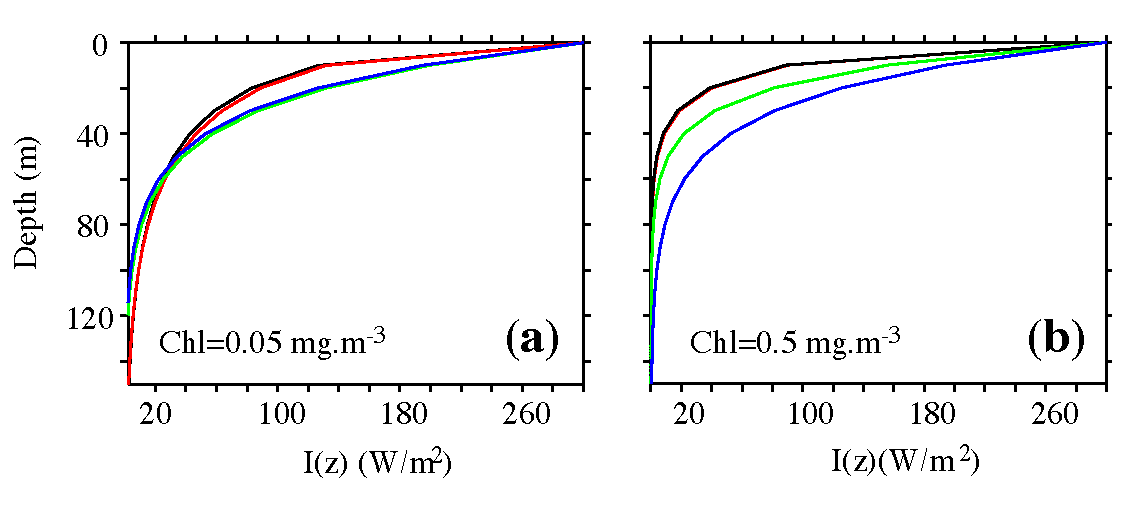
\includegraphics[width=0.66\textwidth]{TRA_Irradiance}
  \caption[Penetration profile of the downward solar irradiance calculated by four models]{
    Penetration profile of the downward solar irradiance calculated by four models.
    Two waveband chlorophyll-independent formulation (blue),
    a chlorophyll-dependent monochromatic formulation (green),
    4 waveband RGB formulation (red),
    61 waveband Morel (1988) formulation (black) for a chlorophyll concentration of
    (a) Chl=0.05 $mg/m^3$ and (b) Chl=0.5 $mg/m^3$.
    From \citet{lengaigne.menkes.ea_CD07}.}
  \label{fig:TRA_qsr_irradiance}
\end{figure}

%% =================================================================================================
\subsection[Bottom boundary condition (\textit{trabbc.F90}) - \forcode{ln_trabbc})]{Bottom boundary condition (\protect\mdl{trabbc} - \protect\np{ln_trabbc}{ln\_trabbc})}
\label{subsec:TRA_bbc}

\begin{listing}
  \nlst{nambbc}
  \caption{\forcode{&nambbc}}
  \label{lst:nambbc}
\end{listing}

\begin{figure}
  \centering
  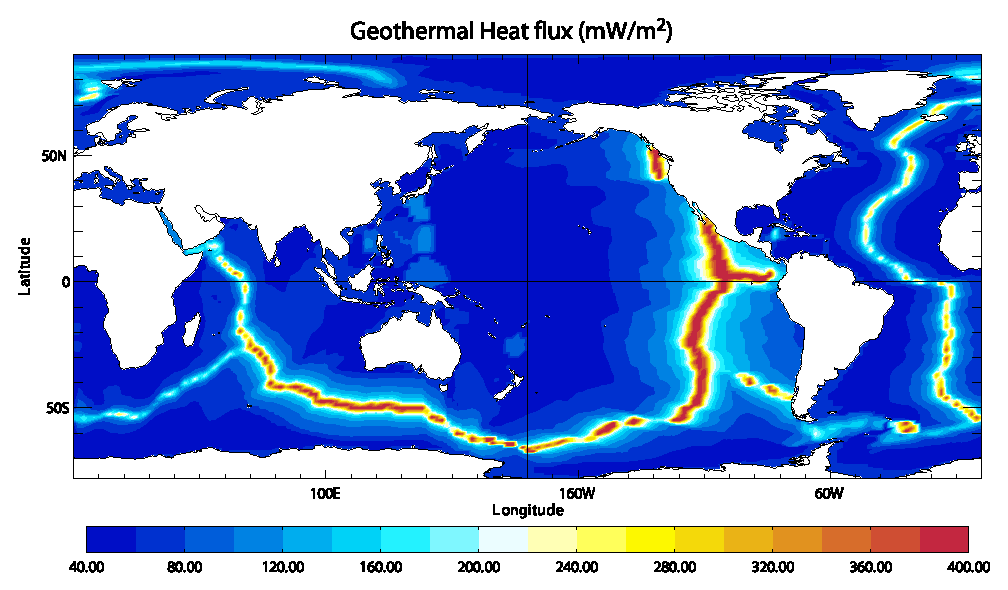
\includegraphics[width=0.66\textwidth]{TRA_geoth}
  \caption[Geothermal heat flux]{
    Geothermal Heat flux (in $mW.m^{-2}$) used by \cite{emile-geay.madec_OS09}.
    It is inferred from the age of the sea floor and the formulae of \citet{stein.stein_N92}.}
  \label{fig:TRA_geothermal}
\end{figure}

Usually it is assumed that there is no exchange of heat or salt through the ocean bottom,
\ie\ a no flux boundary condition is applied on active tracers at the bottom.
This is the default option in \NEMO, and it is implemented using the masking technique.
However, there is a non-zero heat flux across the seafloor that
is associated with solid earth cooling.
This flux is weak compared to surface fluxes
(a mean global value of $\sim 0.1 \, W/m^2$ \citep{stein.stein_N92}),
but it warms systematically the ocean and acts on the densest water masses.
Taking this flux into account in a global ocean model increases the deepest overturning cell
(\ie\ the one associated with the Antarctic Bottom Water) by
a few Sverdrups \citep{emile-geay.madec_OS09}.

Options are defined through the \nam{bbc}{bbc} namelist variables.
The presence of geothermal heating is controlled by
setting the namelist parameter \np{ln_trabbc}{ln\_trabbc} to true.
Then, when \np{nn_geoflx}{nn\_geoflx} is set to 1, a constant geothermal heating is introduced whose
value is given by the \np{rn_geoflx_cst}{rn\_geoflx\_cst}, which is also a namelist parameter.
When \np{nn_geoflx}{nn\_geoflx} is set to 2,
a spatially varying geothermal heat flux is introduced which is provided in
the \ifile{geothermal\_heating} NetCDF file
(\autoref{fig:TRA_geothermal}) \citep{emile-geay.madec_OS09}.

%% =================================================================================================
\section[Bottom boundary layer (\textit{trabbl.F90} - \forcode{ln_trabbl})]{Bottom boundary layer (\protect\mdl{trabbl} - \protect\np{ln_trabbl}{ln\_trabbl})}
\label{sec:TRA_bbl}

\begin{listing}
  \nlst{nambbl}
  \caption{\forcode{&nambbl}}
  \label{lst:nambbl}
\end{listing}

Options are defined through the \nam{bbl}{bbl} namelist variables.
In a $z$-coordinate configuration, the bottom topography is represented by a series of discrete steps.
This is not adequate to represent gravity driven downslope flows.
Such flows arise either downstream of sills such as the Strait of Gibraltar or Denmark Strait,
where dense water formed in marginal seas flows into a basin filled with less dense water,
or along the continental slope when dense water masses are formed on a continental shelf.
The amount of entrainment that occurs in these gravity plumes is critical in
determining the density and volume flux of the densest waters of the ocean,
such as Antarctic Bottom Water, or North Atlantic Deep Water.
$z$-coordinate models tend to overestimate the entrainment,
because the gravity flow is mixed vertically by convection as
it goes ''downstairs'' following the step topography,
sometimes over a thickness much larger than the thickness of the observed gravity plume.
A similar problem occurs in the $s$-coordinate when
the thickness of the bottom level varies rapidly downstream of a sill
\citep{willebrand.barnier.ea_PO01}, and the thickness of the plume is not resolved.

The idea of the bottom boundary layer (BBL) parameterisation, first introduced by
\citet{beckmann.doscher_JPO97},
is to allow a direct communication between two adjacent bottom cells at different levels,
whenever the densest water is located above the less dense water.
The communication can be by a diffusive flux (diffusive BBL),
an advective flux (advective BBL), or both.
In the current implementation of the BBL, only the tracers are modified, not the velocities.
Furthermore, it only connects ocean bottom cells,
and therefore does not include all the improvements introduced by \citet{campin.goosse_T99}.

%% =================================================================================================
\subsection[Diffusive bottom boundary layer (\forcode{nn_bbl_ldf=1})]{Diffusive bottom boundary layer (\protect\np[=1]{nn_bbl_ldf}{nn\_bbl\_ldf})}
\label{subsec:TRA_bbl_diff}

When applying sigma-diffusion
(\np[=.true.]{ln_trabbl}{ln\_trabbl} and \np{nn_bbl_ldf}{nn\_bbl\_ldf} set to 1),
the diffusive flux between two adjacent cells at the ocean floor is given by
\[
  % \label{eq:TRA_bbl_diff}
  \vect F_\sigma = A_l^\sigma \, \nabla_\sigma T
\]
with $\nabla_\sigma$ the lateral gradient operator taken between bottom cells,
and $A_l^\sigma$ the lateral diffusivity in the BBL.
Following \citet{beckmann.doscher_JPO97}, the latter is prescribed with a spatial dependence,
\ie\ in the conditional form
\begin{equation}
  \label{eq:TRA_bbl_coef}
  A_l^\sigma (i,j,t) =
      \begin{cases}
        A_{bbl} & \text{if~} \nabla_\sigma \rho \cdot \nabla H < 0 \\
        0      & \text{otherwise}
      \end{cases}
\end{equation}
where $A_{bbl}$ is the BBL diffusivity coefficient,
given by the namelist parameter \np{rn_ahtbbl}{rn\_ahtbbl} and
usually set to a value much larger than the one used for lateral mixing in the open ocean.
The constraint in \autoref{eq:TRA_bbl_coef} implies that sigma-like diffusion only occurs when
the density above the sea floor, at the top of the slope, is larger than in the deeper ocean
(see green arrow in \autoref{fig:TRA_bbl}).
In practice, this constraint is applied separately in the two horizontal directions,
and the density gradient in \autoref{eq:TRA_bbl_coef} is evaluated with the log gradient formulation:
\[
  % \label{eq:TRA_bbl_Drho}
  \nabla_\sigma \rho / \rho = \alpha \, \nabla_\sigma T + \beta \, \nabla_\sigma S
\]
where $\rho$, $\alpha$ and $\beta$ are functions of
$\overline T^\sigma$, $\overline S^\sigma$ and $\overline H^\sigma$,
the along bottom mean temperature, salinity and depth, respectively.

%% =================================================================================================
\subsection[Advective bottom boundary layer (\forcode{nn_bbl_adv=1,2})]{Advective bottom boundary layer (\protect\np[=1,2]{nn_bbl_adv}{nn\_bbl\_adv})}
\label{subsec:TRA_bbl_adv}

%\sgacomment{
%  "downsloping flow" has been replaced by "downslope flow" in the following
%  if this is not what is meant then "downwards sloping flow" is also a possibility"
%}

\begin{figure}
  \centering
  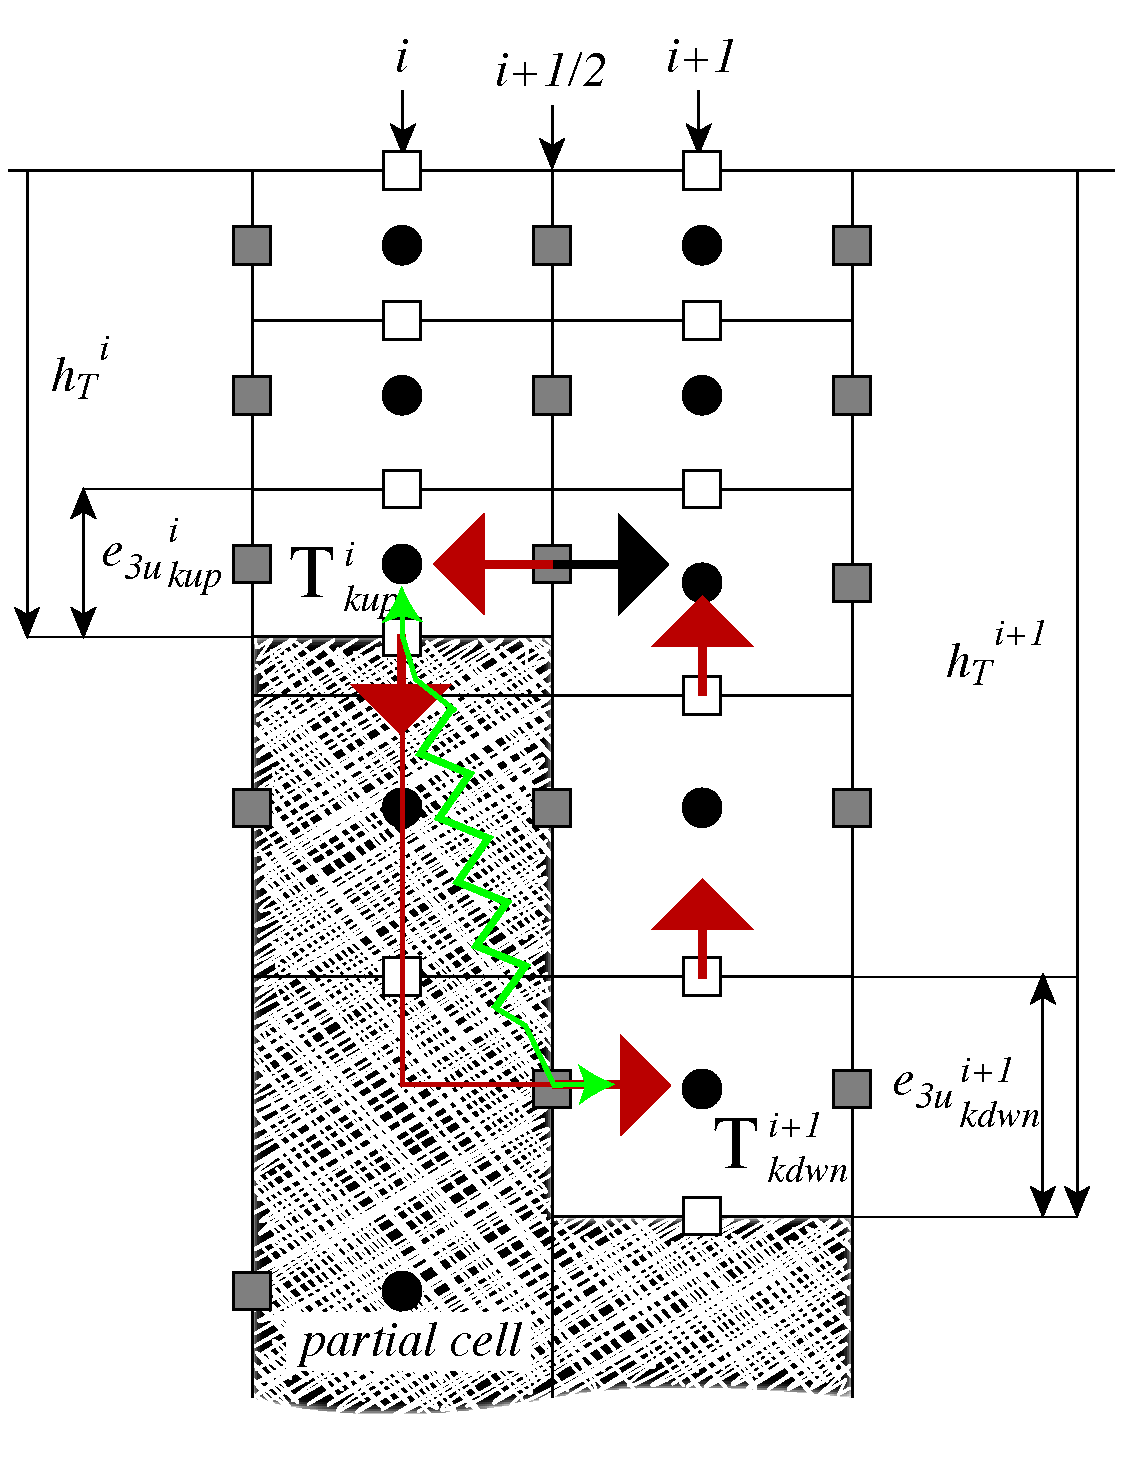
\includegraphics[width=0.33\textwidth]{TRA_BBL_adv}
  \caption[Advective/diffusive bottom boundary layer]{
    Advective/diffusive Bottom Boundary Layer.
    The BBL parameterisation is activated when $\rho^i_{kup}$ is larger than $\rho^{i + 1}_{kdnw}$.
    Red arrows indicate the additional overturning circulation due to the advective BBL.
    The transport of the downslope flow is defined either
    as the transport of the bottom ocean cell (black arrow),
    or as a function of the along slope density gradient.
    The green arrow indicates the diffusive BBL flux directly connecting
    $kup$ and $kdwn$ ocean bottom cells.}
  \label{fig:TRA_bbl}
\end{figure}

%!!      nn_bbl_adv = 1   use of the ocean velocity as bbl velocity
%!!      nn_bbl_adv = 2   follow Campin and Goosse (1999) implentation
%!!        i.e. transport proportional to the along-slope density gradient

\cmtgm{This section has to be really written}

When applying an advective BBL (\np[=1..2]{nn_bbl_adv}{nn\_bbl\_adv}),
an overturning circulation is added which connects two adjacent bottom grid-points only if
dense water overlies less dense water on the slope.
The density difference causes dense water to move down the slope.

\begin{description}
\item [{\np[=1]{nn_bbl_adv}{nn\_bbl\_adv}}] the downslope velocity is chosen to
  be the Eulerian ocean velocity just above the topographic step
  (see black arrow in \autoref{fig:TRA_bbl}) \citep{beckmann.doscher_JPO97}.
  It is a \textit{conditional advection}, that is,
  advection is allowed only if dense water overlies less dense water on the slope
  (\ie\ $\nabla_\sigma \rho \cdot \nabla H < 0$) and if the velocity is directed towards greater depth
  (\ie\ $\vect U \cdot \nabla H > 0$).
\item [{\np[=2]{nn_bbl_adv}{nn\_bbl\_adv}}] the downslope velocity is chosen to be proportional to
  $\Delta \rho$, the density difference between the higher cell and lower cell densities
  \citep{campin.goosse_T99}.
  The advection is allowed only  if dense water overlies less dense water on the slope
  (\ie\ $\nabla_\sigma \rho \cdot \nabla H < 0$).
  For example, the resulting transport of the downslope flow, here in the $i$-direction
  (\autoref{fig:TRA_bbl}), is simply given by the following expression:
  \[
    % \label{eq:TRA_bbl_Utr}
    u^{tr}_{bbl} = \gamma g \frac{\Delta \rho}{\rho_o} e_{1u} \, min ({e_{3u}}_{kup},{e_{3u}}_{kdwn})
  \]
  where $\gamma$, expressed in seconds, is the coefficient of proportionality provided as
  \np{rn_gambbl}{rn\_gambbl}, a namelist parameter, and
  \textit{kup} and \textit{kdwn} are the vertical index of the higher and lower cells, respectively.
  The parameter $\gamma$ should take a different value for each bathymetric step, but for simplicity,
  and because no direct estimation of this parameter is available, a uniform value has been assumed.
  The possible values for $\gamma$ range between 1 and $10~s$ \citep{campin.goosse_T99}.
\end{description}

Scalar properties are advected by this additional transport $(u^{tr}_{bbl},v^{tr}_{bbl})$ using
the upwind scheme.
Such a diffusive advective scheme has been chosen to mimic the entrainment between
the downslope plume and the surrounding water at intermediate depths.
The entrainment is replaced by the vertical mixing implicit in the advection scheme.
Let us consider as an example the case displayed in \autoref{fig:TRA_bbl} where
the density at level $(i,kup)$ is larger than the one at level $(i,kdwn)$.
The advective BBL scheme modifies the tracer time tendency of
the ocean cells near the topographic step by the downslope flow \autoref{eq:TRA_bbl_dw},
the horizontal \autoref{eq:TRA_bbl_hor} and the upward \autoref{eq:TRA_bbl_up} return flows as follows:
\begin{alignat}{5}
  \label{eq:TRA_bbl_dw}
  \partial_t T^{do}_{kdw} &\equiv \partial_t T^{do}_{kdw} &&+ \frac{u^{tr}_{bbl}}{{b_t}^{do}_{kdw}} &&\lt( T^{sh}_{kup} - T^{do}_{kdw} \rt) \\
  \label{eq:TRA_bbl_hor}
  \partial_t T^{sh}_{kup} &\equiv \partial_t T^{sh}_{kup} &&+ \frac{u^{tr}_{bbl}}{{b_t}^{sh}_{kup}} &&\lt( T^{do}_{kup} - T^{sh}_{kup} \rt) \\
  \shortintertext{and for $k =kdw-1,\;..., \; kup$ :}
  \label{eq:TRA_bbl_up}
  \partial_t T^{do}_{k}   &\equiv \partial_t S^{do}_{k}   &&+ \frac{u^{tr}_{bbl}}{{b_t}^{do}_{k}}   &&\lt( T^{do}_{k +1} - T^{sh}_{k}   \rt)
\end{alignat}
where $b_t$ is the $T$-cell volume.

Note that the BBL transport, $(u^{tr}_{bbl},v^{tr}_{bbl})$, is available in the model outputs.
It has to be used to compute the effective velocity as well as the effective overturning circulation.

%% =================================================================================================
\section[Tracer damping (\textit{tradmp.F90})]{Tracer damping (\protect\mdl{tradmp})}
\label{sec:TRA_dmp}

\begin{listing}
  \nlst{namtra_dmp}
  \caption{\forcode{&namtra_dmp}}
  \label{lst:namtra_dmp}
\end{listing}

In some applications it can be useful to add a Newtonian damping term into
the temperature and salinity equations:
\begin{equation}
  \label{eq:TRA_dmp}
    \pd[T]{t} = \cdots - \gamma (T - T_o) \qquad \pd[S]{t} = \cdots - \gamma (S - S_o)
\end{equation}
where $\gamma$ is the inverse of a time scale,
and $T_o$ and $S_o$ are given temperature and salinity fields (usually a climatology).
Options are defined through the \nam{tra_dmp}{tra\_dmp} namelist variables.
The restoring term is added when the namelist parameter \np{ln_tradmp}{ln\_tradmp} is set to true.
It also requires that both \np{ln_tsd_init}{ln\_tsd\_init} and
\np{ln_tsd_dmp}{ln\_tsd\_dmp} are set to true in \nam{tsd}{tsd} namelist as well as
\np{sn_tem}{sn\_tem} and \np{sn_sal}{sn\_sal} structures are correctly set
(\ie\ that $T_o$ and $S_o$ are provided in input files and read using \mdl{fldread},
see \autoref{subsec:SBC_fldread}).
The restoring coefficient $\gamma$ is a three-dimensional array read in during
the \rou{tra\_dmp\_init} routine.
The file name is specified by the namelist variable \np{cn_resto}{cn\_resto}.
The \texttt{DMP\_TOOLS} are provided to allow users to generate the netcdf file.

The two main cases in which \autoref{eq:TRA_dmp} is used are
\begin{enumerate*}[label=(\textit{\alph*})]
\item the specification of the boundary conditions along
  artificial walls of a limited domain basin and
\item the computation of the velocity field associated with a given $T$-$S$ field
  (for example to build the initial state of a prognostic simulation,
  or to use the resulting velocity field for a passive tracer study).
\end{enumerate*}
The first case applies to regional models that have artificial walls instead of open boundaries.
In the vicinity of these walls, $\gamma$ takes large values (equivalent to a time scale of a few days)
whereas it is zero in the interior of the model domain.
The second case corresponds to the use of the robust diagnostic method \citep{sarmiento.bryan_JGR82}.
It allows us to find the velocity field consistent with the model dynamics whilst
having a $T$, $S$ field close to a given climatological field ($T_o$, $S_o$).

The robust diagnostic method is very efficient in preventing temperature drift in
intermediate waters but it produces artificial sources of heat and salt within the ocean.
It also has undesirable effects on the ocean convection.
It tends to prevent deep convection and subsequent deep-water formation,
by stabilising the water column too much.

The namelist parameter \np{nn_zdmp}{nn\_zdmp} sets whether the damping should be applied in
the whole water column or only below the mixed layer (defined either on a density or $S_o$ criterion).
It is common to set the damping to zero in the mixed layer as the adjustment time scale is short here
\citep{madec.delecluse.ea_JPO96}.

For generating \ifile{resto},
see the documentation for the DMP tools provided with the source code under \path{./tools/DMP_TOOLS}.

%% =================================================================================================
\section[Tracer time evolution (\textit{tranxt.F90})]{Tracer time evolution (\protect\mdl{tranxt})}
\label{sec:TRA_nxt}

Options are defined through the \nam{dom}{dom} namelist variables.
The general framework for tracer time stepping is a modified leap-frog scheme
\citep{leclair.madec_OM09}, \ie\ a three level centred time scheme associated with
a Asselin time filter (cf. \autoref{sec:TD_mLF}):
\begin{equation}
  \label{eq:TRA_nxt}
  \begin{alignedat}{5}
    &(e_{3t}T)^{t + \rdt} &&= (e_{3t}T)_f^{t - \rdt} &&+ 2 \, \rdt \,e_{3t}^t \ \text{RHS}^t \\
    &(e_{3t}T)_f^t        &&= (e_{3t}T)^t            &&+ \, \gamma \, \lt[ (e_{3t}T)_f^{t - \rdt} - 2(e_{3t}T)^t + (e_{3t}T)^{t + \rdt} \rt] \\
    &                     &&                         &&- \, \gamma \, \rdt \, \lt[ Q^{t + \rdt/2} - Q^{t - \rdt/2} \rt]
  \end{alignedat}
\end{equation}
where RHS is the right hand side of the temperature equation,
the subscript $f$ denotes filtered values, $\gamma$ is the Asselin coefficient,
and $S$ is the total forcing applied on $T$ (\ie\ fluxes plus content in mass exchanges).
$\gamma$ is initialized as \np{rn_atfp}{rn\_atfp}, its default value is \forcode{10.e-3}.
Note that the forcing correction term in the filter is not applied in linear free surface
(\jp{ln\_linssh}\forcode{=.true.}) (see \autoref{subsec:TRA_sbc}).
Not also that in constant volume case, the time stepping is performed on $T$,
not on its content, $e_{3t}T$.

When the vertical mixing is solved implicitly,
the update of the \textit{next} tracer fields is done in \mdl{trazdf} module.
In this case only the swapping of arrays and the Asselin filtering is done in the \mdl{tranxt} module.

In order to prepare for the computation of the \textit{next} time step,
a swap of tracer arrays is performed: $T^{t - \rdt} = T^t$ and $T^t = T_f$.

%% =================================================================================================
\section[Equation of state (\textit{eosbn2.F90})]{Equation of state (\protect\mdl{eosbn2})}
\label{sec:TRA_eosbn2}

\begin{listing}
  \nlst{nameos}
  \caption{\forcode{&nameos}}
  \label{lst:nameos}
\end{listing}

%% =================================================================================================
\subsection[Equation of seawater (\forcode{ln_}\{\forcode{teos10,eos80,seos}\})]{Equation of seawater (\protect\np{ln_teos10}{ln\_teos10}, \protect\np{ln_teos80}{ln\_teos80}, or \protect\np{ln_seos}{ln\_seos})}
\label{subsec:TRA_eos}

The \textbf{E}quation \textbf{O}f \textbf{S}eawater (EOS) is
an empirical nonlinear thermodynamic relationship linking
seawater density, $\rho$, to a number of state variables,
most typically temperature, salinity and pressure.
Because density gradients control the pressure gradient force through the hydrostatic balance,
the equation of state provides a fundamental bridge between
the distribution of active tracers and the fluid dynamics.
Nonlinearities of the EOS are of major importance, in particular influencing the circulation through
determination of the static stability below the mixed layer,
thus controlling rates of exchange between the atmosphere and the ocean interior
\citep{roquet.madec.ea_JPO15}.
Therefore an accurate EOS based on either the 1980 equation of state
(EOS-80, \cite{fofonoff.millard_bk83}) or TEOS-10 \citep{ioc.iapso_bk10} standards should
be used anytime a simulation of the real ocean circulation is attempted \citep{roquet.madec.ea_JPO15}.
The use of TEOS-10 is highly recommended because
\begin{enumerate*}[label=(\textit{\roman*})]
\item it is the new official EOS,
\item it is more accurate, being based on an updated database of laboratory measurements, and
\item it uses Conservative Temperature and Absolute Salinity
  (instead of potential temperature and practical salinity for EOS-80),
  both variables being more suitable for use as model variables
  \citep{ioc.iapso_bk10, graham.mcdougall_JPO13}.
\end{enumerate*}
EOS-80 is an obsolescent feature of the \NEMO\ system, kept only for backward compatibility.
For process studies, it is often convenient to use an approximation of the EOS.
To that purposed, a simplified EOS (S-EOS) inspired by \citet{vallis_bk06} is also available.

In the computer code, a density anomaly, $d_a = \rho / \rho_o - 1$, is computed,
with $\rho_o$ a reference density.
Called \textit{rau0} in the code,
$\rho_o$ is set in \mdl{phycst} to a value of \texttt{1,026} $Kg/m^3$.
This is a sensible choice for the reference density used in a Boussinesq ocean climate model,
as, with the exception of only a small percentage of the ocean,
density in the World Ocean varies by no more than 2\% from that value \citep{gill_bk82}.

Options which control the EOS used are defined through the \nam{eos}{eos} namelist variables.

\begin{description}
\item [{\np[=.true.]{ln_teos10}{ln\_teos10}}] the polyTEOS10-bsq equation of seawater
  \citep{roquet.madec.ea_OM15} is used.
  The accuracy of this approximation is comparable to the TEOS-10 rational function approximation,
  but it is optimized for a Boussinesq fluid and
  the polynomial expressions have simpler and more computationally efficient expressions for
  their derived quantities which make them more adapted for use in ocean models.
  Note that a slightly higher precision polynomial form is now used
  replacement of the TEOS-10 rational function approximation for hydrographic data analysis
  \citep{ioc.iapso_bk10}.
  A key point is that conservative state variables are used:
  Absolute Salinity (unit: $g/kg$, notation: $S_A$) and
  Conservative Temperature (unit: $\deg{C}$, notation: $\Theta$).
  The pressure in decibars is approximated by the depth in meters.
  With TEOS10, the specific heat capacity of sea water, $C_p$, is a constant.
  It is set to $C_p$ = 3991.86795711963 $J.Kg^{-1}.\deg{K}^{-1}$,
  according to \citet{ioc.iapso_bk10}.
  Choosing polyTEOS10-bsq implies that the state variables used by the model are $\Theta$ and $S_A$.
  In particular, the initial state defined by the user have to be given as
  \textit{Conservative} Temperature and \textit{Absolute} Salinity.
  In addition, when using TEOS10, the Conservative SST is converted to potential SST prior to
  either computing the air-sea and ice-sea fluxes (forced mode) or
  sending the SST field to the atmosphere (coupled mode).
\item [{\np[=.true.]{ln_eos80}{ln\_eos80}}] the polyEOS80-bsq equation of seawater is used.
  It takes the same polynomial form as the polyTEOS10,
  but the coefficients have been optimized to accurately fit EOS80 (Roquet, personal comm.).
  The state variables used in both the EOS80 and the ocean model are:
  the Practical Salinity (unit: $psu$, notation: $S_p$) and
  Potential Temperature (unit: $\deg{C}$, notation: $\theta$).
  The pressure in decibars is approximated by the depth in meters.
  With EOS, the specific heat capacity of sea water, $C_p$, is a function of
  temperature, salinity and pressure \citep{fofonoff.millard_bk83}.
  Nevertheless, a severe assumption is made in order to have a heat content ($C_p T_p$) which
  is conserved by the model: $C_p$ is set to a constant value, the TEOS10 value.
\item [{\np[=.true.]{ln_seos}{ln\_seos}}] a simplified EOS (S-EOS) inspired by
  \citet{vallis_bk06} is chosen,
  the coefficients of which has been optimized to fit the behavior of TEOS10 (Roquet, personal comm.)
  (see also \citet{roquet.madec.ea_JPO15}).
  It provides a simplistic linear representation of both cabbeling and thermobaricity effects which
  is enough for a proper treatment of the EOS in theoretical studies \citep{roquet.madec.ea_JPO15}.
  With such an equation of state there is no longer a distinction between \textit{conservative} and
  \textit{potential} temperature, as well as between \textit{absolute} and
  \textit{practical} salinity.
  S-EOS takes the following expression:
  \begin{gather*}
    % \label{eq:TRA_S-EOS}
    d_a(T,S,z) = \frac{1}{\rho_o} \big[ - a_0 \; ( 1 + 0.5 \; \lambda_1 \; T_a + \mu_1 \; z ) * T_a \big.
                                        + b_0 \; ( 1 - 0.5 \; \lambda_2 \; S_a - \mu_2 \; z ) * S_a
                                  \big. - \nu \;                           T_a                  S_a \big] \\
    \text{with~} T_a = T - 10 \, ; \, S_a = S - 35 \, ; \, \rho_o = 1026~Kg/m^3
  \end{gather*}
  where the computer name of the coefficients as well as their standard value are given in
  \autoref{tab:TRA_SEOS}.
  In fact, when choosing S-EOS, various approximation of EOS can be specified simply by
  changing the associated coefficients.
  Setting to zero the two thermobaric coefficients $(\mu_1,\mu_2)$
  remove thermobaric effect from S-EOS.
  Setting to zero the three cabbeling coefficients $(\lambda_1,\lambda_2,\nu)$
  remove   cabbeling effect from S-EOS.
  Keeping non-zero value to $a_0$ and $b_0$ provide a linear EOS function of T and S.
\end{description}

\begin{table}
  \centering
  \begin{tabular}{|l|l|l|l|}
    \hline
    coeff.      & computer name                & S-EOS            & description                     \\
    \hline
    $a_0      $ & \np{rn_a0}{rn\_a0}           & $1.6550~10^{-1}$ & linear thermal expansion coeff. \\
    \hline
    $b_0      $ & \np{rn_b0}{rn\_b0}           & $7.6554~10^{-1}$ & linear haline  expansion coeff. \\
    \hline
    $\lambda_1$ & \np{rn_lambda1}{rn\_lambda1} & $5.9520~10^{-2}$ & cabbeling coeff. in $T^2$       \\
    \hline
    $\lambda_2$ & \np{rn_lambda2}{rn\_lambda2} & $5.4914~10^{-4}$ & cabbeling coeff. in $S^2$       \\
    \hline
    $\nu      $ & \np{rn_nu}{rn\_nu}           & $2.4341~10^{-3}$ & cabbeling coeff. in $T \, S$    \\
    \hline
    $\mu_1    $ & \np{rn_mu1}{rn\_mu1}         & $1.4970~10^{-4}$ & thermobaric coeff. in T         \\
    \hline
    $\mu_2    $ & \np{rn_mu2}{rn\_mu2}         & $1.1090~10^{-5}$ & thermobaric coeff. in S         \\
    \hline
  \end{tabular}
  \caption{Standard value of S-EOS coefficients}
  \label{tab:TRA_SEOS}
\end{table}

%% =================================================================================================
\subsection[Brunt-V\"{a}is\"{a}l\"{a} frequency]{Brunt-V\"{a}is\"{a}l\"{a} frequency}
\label{subsec:TRA_bn2}

An accurate computation of the ocean stability (i.e. of $N$, the Brunt-V\"{a}is\"{a}l\"{a} frequency) is of paramount importance as determine the ocean stratification and
is used in several ocean parameterisations
(namely TKE, GLS, Richardson number dependent vertical diffusion, enhanced vertical diffusion,
non-penetrative convection, tidal mixing  parameterisation, iso-neutral diffusion).
In particular, $N^2$ has to be computed at the local pressure
(pressure in decibar being approximated by the depth in meters).
The expression for $N^2$  is given by:
\[
  % \label{eq:TRA_bn2}
  N^2 = \frac{g}{e_{3w}} \lt( \beta \; \delta_{k + 1/2}[S] - \alpha \; \delta_{k + 1/2}[T] \rt)
\]
where $(T,S) = (\Theta,S_A)$ for TEOS10, $(\theta,S_p)$ for TEOS-80, or $(T,S)$ for S-EOS, and,
$\alpha$ and $\beta$ are the thermal and haline expansion coefficients.
The coefficients are a polynomial function of temperature, salinity and depth which
expression depends on the chosen EOS.
They are computed through \textit{eos\_rab}, a \fortran\ function that can be found in \mdl{eosbn2}.

%% =================================================================================================
\subsection{Freezing point of seawater}
\label{subsec:TRA_fzp}

The freezing point of seawater is a function of salinity and pressure \citep{fofonoff.millard_bk83}:
\begin{equation}
  \label{eq:TRA_eos_fzp}
  \begin{gathered}
    T_f (S,p) = \lt( a + b \, \sqrt{S} + c \, S \rt) \, S + d \, p \\
    \text{where~} a = -0.0575, \, b = 1.710523~10^{-3}, \, c = -2.154996~10^{-4} \text{and~} d = -7.53~10^{-3}
    \end{gathered}
\end{equation}

\autoref{eq:TRA_eos_fzp} is only used to compute the potential freezing point of sea water
(\ie\ referenced to the surface $p = 0$),
thus the pressure dependent terms in \autoref{eq:TRA_eos_fzp} (last term) have been dropped.
The freezing point is computed through \textit{eos\_fzp},
a \fortran\ function that can be found in \mdl{eosbn2}.

%% =================================================================================================
%\subsection{Potential Energy anomalies}
%\label{subsec:TRA_bn2}

%    =====>>>>> TO BE written

%% =================================================================================================
\section[Horizontal derivative in \textit{zps}-coordinate (\textit{zpshde.F90})]{Horizontal derivative in \textit{zps}-coordinate (\protect\mdl{zpshde})}
\label{sec:TRA_zpshde}

\cmtgm{STEVEN: to be consistent with earlier discussion of differencing and averaging operators,
I've changed "derivative" to "difference" and "mean" to "average"}

With partial cells (\np[=.true.]{ln_zps}{ln\_zps}) at bottom and top
(\np[=.true.]{ln_isfcav}{ln\_isfcav}),
in general, tracers in horizontally adjacent cells live at different depths.
Horizontal gradients of tracers are needed for horizontal diffusion
(\mdl{traldf} module) and the hydrostatic pressure gradient calculations (\mdl{dynhpg} module).
The partial cell properties at the top (\np[=.true.]{ln_isfcav}{ln\_isfcav}) are computed in
the same way as for the bottom.
So, only the bottom interpolation is explained below.

Before taking horizontal gradients between the tracers next to the bottom,
a linear interpolation in the vertical is used to approximate the deeper tracer as if
it actually lived at the depth of the shallower tracer point (\autoref{fig:TRA_Partial_step_scheme}).
For example, for temperature in the $i$-direction the needed interpolated temperature,
$\widetilde T$, is:

\begin{figure}
  \centering
  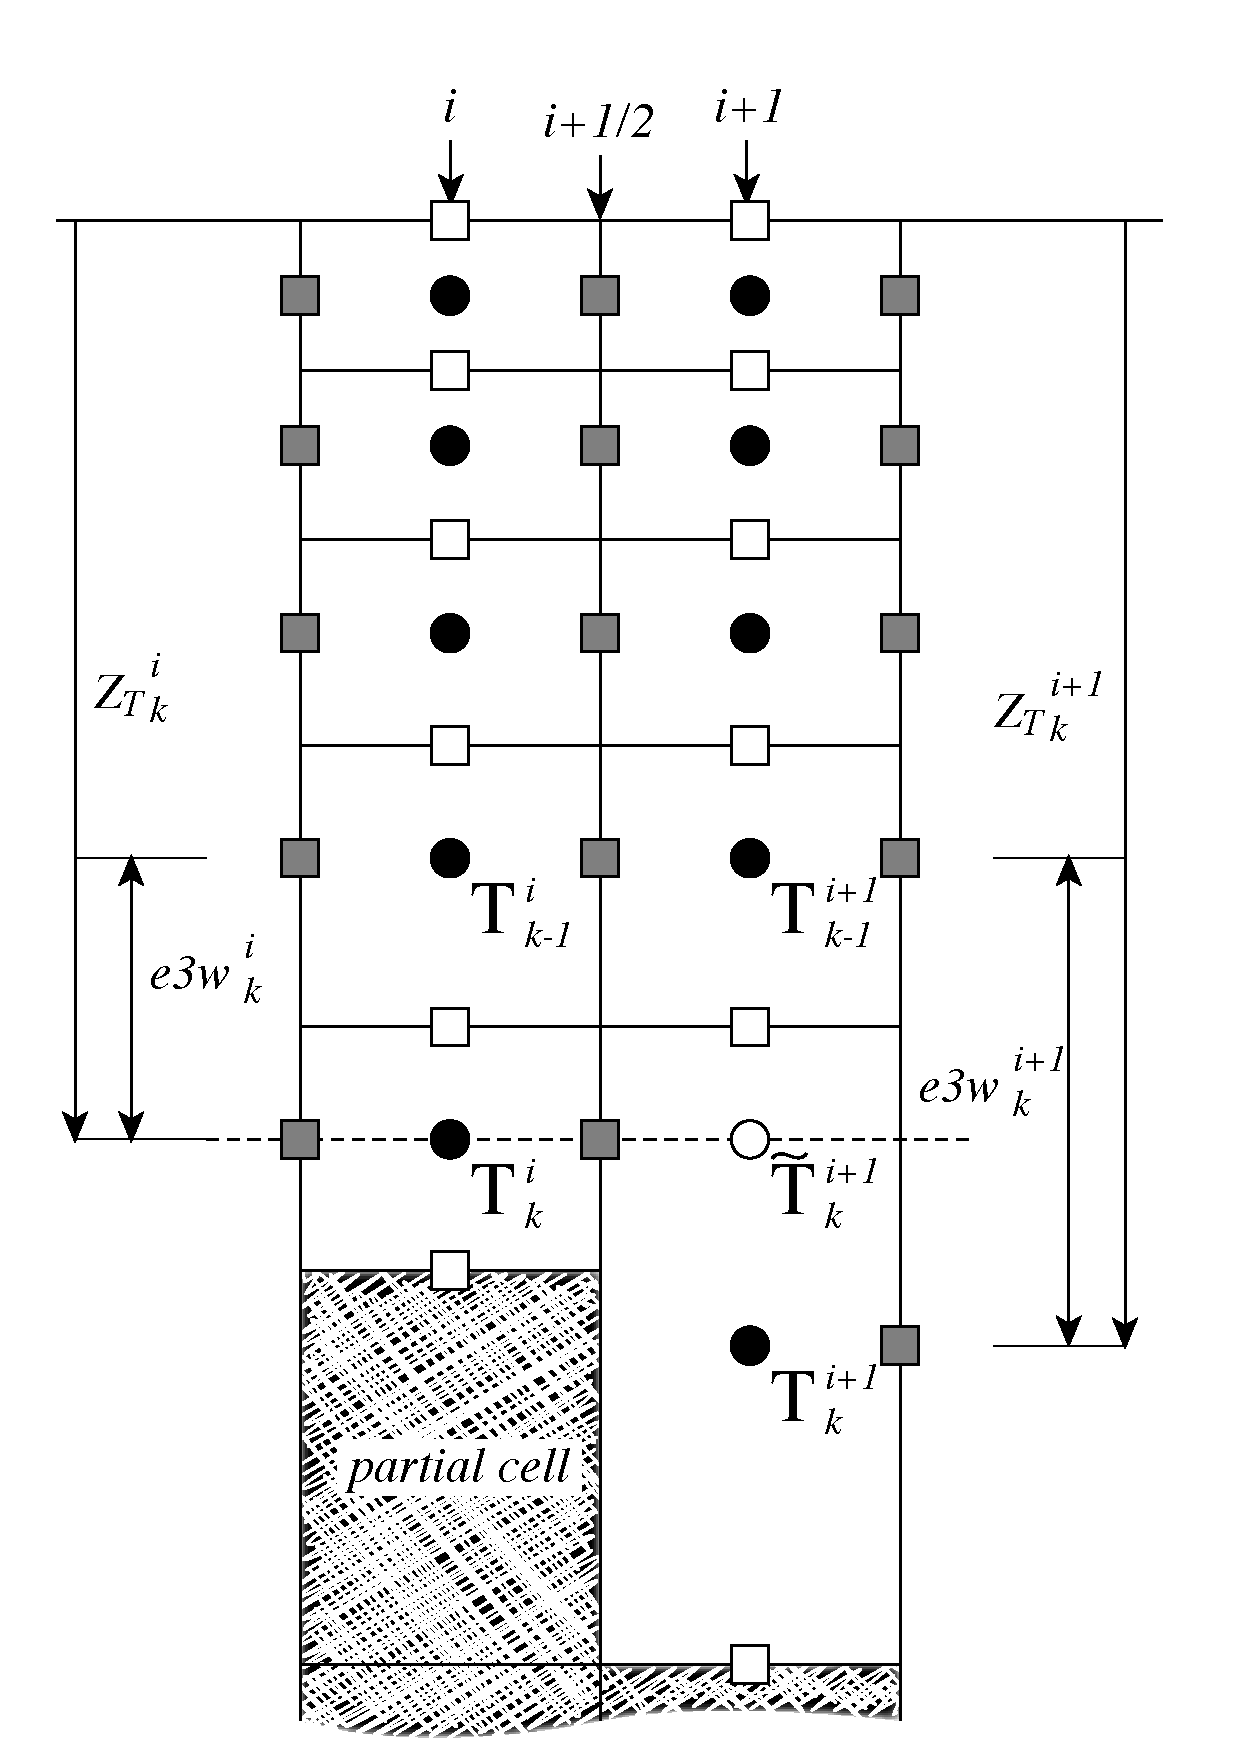
\includegraphics[width=0.33\textwidth]{TRA_partial_step_scheme}
  \caption[Discretisation of the horizontal difference and average of tracers in
  the $z$-partial step coordinate]{
    Discretisation of the horizontal difference and average of tracers in
    the $z$-partial step coordinate (\protect\np[=.true.]{ln_zps}{ln\_zps}) in
    the case $(e3w_k^{i + 1} - e3w_k^i) > 0$.
    A linear interpolation is used to estimate $\widetilde T_k^{i + 1}$,
    the tracer value at the depth of the shallower tracer point of the two adjacent bottom $T$-points.
    The horizontal difference is then given by:
    $\delta_{i + 1/2} T_k = \widetilde T_k^{\, i + 1} -T_k^{\, i}$ and the average by:
    $\overline T_k^{\, i + 1/2} = (\widetilde T_k^{\, i + 1/2} - T_k^{\, i}) / 2$.}
  \label{fig:TRA_Partial_step_scheme}
\end{figure}

\[
  \widetilde T = \lt\{
    \begin{alignedat}{2}
      &T^{\, i + 1} &-\frac{ \lt( e_{3w}^{i + 1} -e_{3w}^i \rt) }{ e_{3w}^{i + 1} } \; \delta_k T^{i + 1}
      & \quad \text{if $e_{3w}^{i + 1} \geq e_{3w}^i$} \\
      &T^{\, i}     &+\frac{ \lt( e_{3w}^{i + 1} -e_{3w}^i \rt )}{e_{3w}^i       } \; \delta_k T^{i + 1}
      & \quad \text{if $e_{3w}^{i + 1} <    e_{3w}^i$}
    \end{alignedat}
  \rt.
\]
and the resulting forms for the horizontal difference and the horizontal average value of
$T$ at a $U$-point are:
\begin{equation}
  \label{eq:TRA_zps_hde}
  \begin{split}
    \delta_{i + 1/2} T       &=
    \begin{cases}
      \widetilde T - T^i          & \text{if~} e_{3w}^{i + 1} \geq e_{3w}^i \\
      T^{\, i + 1} - \widetilde T & \text{if~} e_{3w}^{i + 1} <    e_{3w}^i
    \end{cases} \\
    \overline T^{\, i + 1/2} &=
    \begin{cases}
      (\widetilde T - T^{\, i}    ) / 2 & \text{if~} e_{3w}^{i + 1} \geq e_{3w}^i \\
      (T^{\, i + 1} - \widetilde T) / 2 & \text{if~} e_{3w}^{i + 1} <   e_{3w}^i
    \end{cases}
  \end{split}
\end{equation}

The computation of horizontal derivative of tracers as well as of density is performed once for all at
each time step in \mdl{zpshde} module and stored in shared arrays to be used when needed.
It has to be emphasized that the procedure used to compute the interpolated density,
$\widetilde \rho$, is not the same as that used for $T$ and $S$.
Instead of forming a linear approximation of density,
we compute $\widetilde \rho$ from the interpolated values of $T$ and $S$,
and the pressure at a $u$-point
(in the equation of state pressure is approximated by depth, see \autoref{subsec:TRA_eos}):
\[
  % \label{eq:TRA_zps_hde_rho}
  \widetilde \rho = \rho (\widetilde T,\widetilde S,z_u) \quad \text{where~} z_u = \min \lt( z_T^{i + 1},z_T^i \rt)
\]

This is a much better approximation as the variation of $\rho$ with depth (and thus pressure)
is highly non-linear with a true equation of state and thus is badly approximated with
a linear interpolation.
This approximation is used to compute both the horizontal pressure gradient (\autoref{sec:DYN_hpg})
and the slopes of neutral surfaces (\autoref{sec:LDF_slp}).

Note that in almost all the advection schemes presented in this chapter,
both averaging and differencing operators appear.
Yet \autoref{eq:TRA_zps_hde} has not been used in these schemes:
in contrast to diffusion and pressure gradient computations,
no correction for partial steps is applied for advection.
The main motivation is to preserve the domain averaged mean variance of the advected field when
using the $2^{nd}$ order centred scheme.
Sensitivity of the advection schemes to the way horizontal averages are performed in
the vicinity of partial cells should be further investigated in the near future.
\cmtgm{gm :   this last remark has to be done}

\subinc{\input{../../global/epilogue}}

\end{document}
